% FYP Final Report — Loss Function Design for Cross-Sectional Stock-Return Prediction
% Converted from Obsidian markdown (paper/已修改/) on 2026-05-11
% Compile with: tectonic main.tex (or xelatex main.tex && bibtex main && xelatex main.tex && xelatex main.tex)

\documentclass[12pt,a4paper]{report}

% === Core packages ===
\usepackage{fontspec}
\usepackage{xeCJK}
\setCJKmainfont{Songti SC}
\setmainfont{Times New Roman}
\usepackage[margin=2.5cm]{geometry}
\usepackage{setspace}
\onehalfspacing

% === Math ===
\usepackage{amsmath,amssymb,mathtools}

% === Tables ===
\usepackage{booktabs}
\usepackage{array}
\usepackage{tabularx}
\usepackage{multirow}
\usepackage{colortbl}
\usepackage{xcolor}

% === Figures ===
\usepackage{graphicx}
\graphicspath{{../figures/}{./figures/}}
\usepackage{float}

% === References & hyperlinks ===
\usepackage[numbers,sort&compress]{natbib}
\usepackage{hyperref}
\hypersetup{
  colorlinks=true,
  linkcolor=blue!60!black,
  citecolor=blue!60!black,
  urlcolor=blue!70!black,
}

% === Code listings ===
\usepackage{listings}
\lstset{
  basicstyle=\ttfamily\small,
  breaklines=true,
  frame=single,
  numbers=left,
  numberstyle=\tiny,
  columns=fullflexible,
  keepspaces=true,
}

% === Highlight macros for tables ===
\definecolor{bestred}{HTML}{FF0000}
\definecolor{secondblue}{HTML}{0000FF}
\definecolor{gaingreen}{HTML}{008000}
\newcommand{\best}[1]{\textcolor{bestred}{\textbf{#1}}}
\newcommand{\second}[1]{\textcolor{secondblue}{\underline{#1}}}
\newcommand{\gain}[1]{\textcolor{gaingreen}{#1}}

% === Misc ===
\usepackage{enumitem}
\usepackage{caption}
\captionsetup{font=small,labelfont=bf}

% ==============================================================================
\begin{document}

% === Title page (exact template format) ===
\begin{titlepage}
  \centering
  \vspace*{3cm}
  {\LARGE\bfseries Loss Function Design for\\Cross-Sectional Stock-Return Prediction\par}
  \vspace{0.5cm}
  {\Large 损失函数设计用于横截面股票收益预测\par}
  \vspace{2.5cm}
  {\large a thesis\\submitted to School of Mathematics \& Physics\\of Xi'an Jiaotong-Liverpool University\\in partial fulfilment for the award of the degree of\par}
  \vspace{1.5cm}
  {\Large\bfseries BSc Applied Mathematics\par}
  \vspace{2cm}
  {\large By\par}
  \vspace{1cm}
  {\Large Roucheng Li\par}
  {\large Student ID: XXXXXXXXX\par}
  \vspace{1cm}
  {\large Supervisor: Dr. XXXX XXXX\par}
  \vspace{2cm}
  {\large May 2026\par}
\end{titlepage}

% Blank page
\thispagestyle{empty}
\cleardoublepage

% === Front matter ===
\pagenumbering{roman}

% Abstract
\chapter*{Abstract}
\section*{}
Cross-sectional stock-return prediction with neural networks commonly optimises Mean Squared Error (MSE) or a close relative, yet the downstream decision --- a long-short portfolio --- depends on the cross-sectional rank of the predictions, not on their calibrated magnitudes. Under this mismatch, a quadratic loss gives disproportionate training weight to heavy-tailed outliers, and the resulting model trades ranking quality for calibration quality that the portfolio does not use. This report asks whether a hybrid loss that combines a directional-accuracy term with a robust magnitude term can outperform both traditional regression losses and pure directional losses under a controlled evaluation protocol.

The study uses a CRSP-style US equity monthly panel with a static protocol: training window \texttt{1990-01} to \texttt{1994-12} (60 monthly cross-sections) and main out-of-sample test window \texttt{1995-01} to \texttt{1996-12} (24 monthly cross-sections). The model is a fixed multi-layer perceptron (MLP) with hidden widths $[64, 32, 16]$, ReLU activations, and dropout $0.2$, consuming 15 model-input columns (see Chapter 4 \S4.4.1 and Appendix B Table B.3). Training uses batch size $1024$ and 20 epochs of Adam; the trained model is then evaluated month-by-month on a top/bottom-10\% signal-tilted long-short portfolio with a 5\% per-name cap. Performance is reported as annualised Sharpe ($\sqrt{12}$-scaled monthly mean/std), cumulative 24-month return, and, for multi-seed phases, the coefficient of variation $\mathrm{CV} = \sigma_S / |\mu_S|$ across three random seeds.

Four comparison phases plus one normalisation probe are run. Within each comparison table, the loss function is the only varying factor; cross-phase comparisons differ in additional dimensions (\S3.8). A Phase 1 single-seed baseline compares seven loss families (MSE, MedSE, MADL, GMADL, IMADL, and two hybrid multiplicative variants). A Phase 2 sweep scans nine parameterised hybrid variants (five additive A-series and four multiplicative M-series). Phase 3 refines the M2-robust loss with a $\gamma$ parameter and evaluates five $\gamma$ settings across three seeds, then extends the comparison to IMADL-m2 $\alpha$, IMADL-GMADL $\beta$, and adaptive-$\lambda$ sweeps under the same multi-seed protocol. Finally, a Phase 4 normalisation probe tests loss-component normalisation on the top three candidates as a diagnostic follow-up.

The multi-seed evidence identifies \texttt{m2\_robust\_gamma07} (multiplicative hybrid with robustness parameter $\gamma = 0.07$) as the best-supported choice. It achieves mean Sharpe $0.9156$, CV $0.1808$, and mean cumulative return $+27.99\%$ across three seeds; no seed produces a negative Sharpe in this configuration, and the result is approximately flat under loss-component normalisation (normalised mean Sharpe $0.9112$). The high-return alternative \texttt{m2\_robust\_gamma10} reaches a mean Sharpe of $1.0043$ but has CV $0.5613$ --- three times that of $\gamma$07 --- and degrades to mean Sharpe $0.4072$ under normalisation; it is only appropriate when higher seed sensitivity is acceptable. The stable fallback \texttt{imadl\_m2\_alpha06}, drawn from an independent parameterisation, achieves mean Sharpe $0.6895$ with CV $0.2443$ and the largest mean cumulative return of the three candidates at $+30.42\%$; it is selected by the stability/return trade-off rather than by Sharpe dominance. Traditional regression losses (MSE, MedSE) and pure directional losses (MADL, GMADL, IMADL) do not produce economically meaningful positive Sharpes in the seed-42 same-window baseline, and the absolute-loss family additionally exhibits very negative point-prediction R\textsuperscript{2} values while retaining competitive ranking performance --- a dissociation between calibration and portfolio quality that the report makes explicit.

Three boundaries constrain the conclusions. First, the evaluation uses a single static 24-month window; the rolling-window extension is listed as future work. Second, multi-seed evaluations use three seeds, which is sufficient to differentiate CV at the order-of-magnitude level but not to bound CV to the second decimal. Third, the loss-component normalisation probe's scale ratios are diagnostics-estimated rather than measured by a per-component logger, which is flagged as a priority instrumentation task. Within these boundaries the report provides a verifiable recommendation --- \texttt{m2\_robust\_gamma07} as the primary loss, with explicit high-return and stable-fallback alternatives --- together with a source-of-truth evidence map that ties every reported number to a named artifact file.

\vspace{5cm}

\noindent \textbf{KEY WORDS}: loss function design; robust regression; MADL; GMADL; cross-sectional stock-return prediction; long-short portfolio; multi-layer perceptron; multi-seed robustness; coefficient of variation; CRSP

\cleardoublepage

% TOC
\tableofcontents
\cleardoublepage

% Lists
\listoffigures
\cleardoublepage
\listoftables
\cleardoublepage

% === Main body ===
\pagenumbering{arabic}
\setcounter{page}{1}

% Chapter 1: Introduction

\chapter{Introduction}
\label{ch1:introduction}

\section{Background and Motivation}
\label{ch1:background}

Machine-learning models are now widely used for cross-sectional stock-return prediction and long-short portfolio construction. In this setting, the loss function is not just a technical training choice: it determines which prediction errors the model treats as important. Yet most return-prediction studies vary architectures and feature sets while keeping the objective at generic regression losses such as Mean Squared Error (MSE) or Mean Absolute Error (MAE).

This default is not fully aligned with the portfolio task. A long-short portfolio depends mainly on the cross-sectional ranking of predictions, not on their calibrated point values, and monthly equity returns are heavy-tailed. A model can therefore reduce MSE while still ranking the most economically relevant names poorly, or devote excessive training weight to noisy tail observations that do not improve portfolio construction.

Existing loss-function families address parts of this problem. Robust losses reduce the influence of heavy-tailed residuals, while directional losses such as MADL and GMADL \cite{ref7, ref8} reward correct return signs and magnitude-weighted directional alignment. What remains less clear is how regression, robust, directional, and hybrid losses compare under the same data, feature input, model, and portfolio rule. This report addresses that gap through a controlled empirical study of loss-function design for portfolio-oriented return prediction.

\section{Research Objectives}
\label{ch1:objectives}

This report has four objectives.
First, it benchmarks standard regression, robust, directional, and initial hybrid losses under a common 24-month out-of-sample protocol.
Second, it develops and evaluates hybrid loss functions that combine a directional component with a robust magnitude component.
Third, it evaluates the most relevant hybrid families under multi-seed conditions, using both mean Sharpe and cross-seed stability to avoid relying on a single favourable run.
Fourth, it checks whether the recommended loss remains approximately stable under a diagnostic loss-component normalisation probe.
The study is deliberately narrow. It fixes the equity universe, X1 feature input, MLP architecture, static 1990--1994 training window, 1995--1996 test window, and long-short portfolio construction. Architecture search, feature-set sensitivity, rolling-window validation, transaction costs, and non-US or non-monthly settings are outside the main claim boundary.

\section{Research Questions}
\label{ch1:questions}

\textbf{RQ1: How does loss choice affect prediction-level and portfolio-level performance under a fixed evaluation protocol?}
This question compares regression, robust, directional, and hybrid losses while holding data, model, and portfolio rule fixed, asking whether calibration metrics ($R^2$) and portfolio metrics (Sharpe) move together or decouple.

\textbf{RQ2: Which hybrid-loss design gives the best supported Sharpe-stability trade-off?}
Among hybrid losses that combine directional alignment with robust magnitude control, this question asks which parameterisation achieves the highest mean Sharpe while maintaining tolerable cross-seed variability.

\textbf{RQ3: Are the leading hybrid-loss candidates approximately stable under diagnostic component normalisation?}
This question tests whether the observed Sharpe ordering is driven by the relative scale of loss components or by a genuine loss-family effect.

Chapter~5 reports the empirical evidence for these questions, and Chapter~6 synthesises the answers.

\section{Contributions and Report Structure}
\label{ch1:contributions}

The report makes four contributions.

\begin{enumerate}
    \item \textbf{A controlled loss-function benchmark} comparing regression, robust, directional, and hybrid losses under a common 24-month protocol.
    \item \textbf{A hybrid-loss design study} developing additive and multiplicative hybrids that combine directional alignment with robust magnitude control.
    \item \textbf{A multi-seed robustness comparison} evaluating leading hybrid candidates using mean Sharpe, cumulative return, and cross-seed stability.
    \item \textbf{A bounded final recommendation} identifying \texttt{m2\_robust\_gamma07} as the best-supported primary choice, with \texttt{m2\_robust\_gamma10} as a higher-return alternative and \texttt{imadl\_m2\_alpha06} as a stable fallback.
\end{enumerate}

The remainder of the report is organised as follows. Chapter~2 reviews return-prediction, robust-regression, and directional-loss literature. Chapter~3 describes the methodology. Chapter~4 documents the data. Chapter~5 presents the empirical results. Chapter~6 answers the research questions, states limitations, and outlines future work.

\cleardoublepage

\chapter{Literature Review}\label{ch:literature_review}

The design space explored in this report sits at the intersection of three strands of literature: (i) machine learning for cross-sectional stock-return prediction, (ii) robust regression under heavy-tailed outcomes, and (iii) trading-aware loss functions that target portfolio rather than point-prediction objectives. This chapter reviews each strand in turn and uses the review to motivate a controlled comparison of regression, robust, directional, and hybrid losses. The project-specific hybrid formulations are defined in Chapter~3 and evaluated in Chapter~5.

\section{Machine Learning for Cross-Sectional Stock-Return Prediction}\label{sec:ml_cross_sectional}

Empirical asset pricing has historically relied on linear factor models in which the expected cross-sectional return is assumed to be a linear function of a small set of pre-specified characteristics. The three-factor model of Fama and French (1993) --- market, size, and book-to-market --- remains the workhorse benchmark, later extended to include momentum, profitability, and investment factors \cite{ref2}. These models succeed as parsimonious explanations but impose a linear structure on a relationship that need not be linear.

Modern machine-learning approaches relax this linearity. Gu, Kelly, and Xiu (2020) construct a comprehensive comparative study across regression trees, gradient boosting, random forests, and deep neural networks on a panel of 94 stock characteristics, and find that deeper non-linear models systematically outperform linear benchmarks out of sample \cite{ref1}. Their follow-up work on autoencoder asset pricing models \cite{ref9} further demonstrates that latent-factor extraction from the same characteristic panel improves pricing accuracy. Han (2021) shows that bimodal return distributions can be exploited by ML models to enhance predictability beyond what linear factor models capture \cite{ref10}. Their key finding --- that model capacity translates into incremental out-of-sample predictive power --- has motivated a wave of MLP, LSTM, and transformer-based architectures applied to return prediction. Daniel and Moskowitz (2016) complement this architectural work on the feature side, isolating cumulative-return and turnover-based predictors that capture medium-term momentum while avoiding short-term reversal \cite{ref3}. Medhat and Schmeling (2021) extend this to short-term momentum signals based on cumulative turnover \cite{ref11}. The feature set X1 used throughout this report (Chapter~4) follows their construction.

The pattern across this literature is informative: essentially every study iterates on architecture and feature construction while holding the training objective fixed, typically at MSE. Because the downstream decision --- a long-short portfolio --- depends on the cross-sectional \textit{ranking} of predictions rather than their calibrated values, and because return distributions deviate substantially from the Gaussian noise assumption implicit in MSE, there is a clear opening to ask whether the fixed choice of MSE is the right one. That question is the starting point of this report.

\section{Heavy-Tailed Returns and the Case for Robust Losses}\label{sec:heavy_tailed_returns}

Equity returns are not Gaussian. Monthly cross-sections contain sporadic observations with returns in excess of $\pm 100\%$ (in the training-era panel used in Chapter~4, the realised monthly return distribution has a standard deviation of roughly $19.5\%$ but a maximum of $+2400\%$ for a single name-month). Four properties of this distribution challenge standard loss functions:

\begin{enumerate}
    \item \textbf{Heavy tails.} Extreme returns occur far more often than a Gaussian model predicts, so the variance of a sample is dominated by a small number of tail observations.
    \item \textbf{Skewness.} Return distributions are often negatively skewed at the individual-stock level, though the training panel's extreme positive tail ($+2400\%$) shows that right-tail outliers also occur. The asymmetry violates the symmetric-noise assumption of MSE.
    \item \textbf{Time-varying volatility.} Volatility clusters, violating the homoskedasticity assumption that underpins MSE's efficiency argument.
    \item \textbf{Idiosyncratic shocks.} Company-specific events (earnings surprises, management changes, regulatory shocks) produce large returns that are unrelated to predictable factors and act as noise from the perspective of a factor-style model.
\end{enumerate}

Under these conditions, a loss function that is quadratic in the residual gives disproportionate weight to a small number of outliers. The trained model fits the noise rather than the predictable component. This is the classical motivation for robust regression --- a line of work that goes back at least to Huber (1964) \cite{refA1} and has been applied extensively to finance whenever heavy tails matter.

Huber loss offers a principled middle ground between quadratic and linear penalisation: for residuals below a threshold $\delta$ the loss behaves like MSE, preserving efficiency under near-Gaussian conditions; for residuals above $\delta$ it behaves like MAE, limiting the influence of any single observation. The resulting M-estimator retains desirable convexity and differentiability properties while being robust to a non-trivial fraction of contamination (see Appendix~A \S~A.1.3 for the closed-form expression).

More aggressive robustness is provided by median-based losses. Median Squared Error (MedSE), $\mathrm{MedSE} = \mathrm{median}_i[(y_i - \hat{y}_i)^2]$, depends only on the central ordered residual and is therefore unaffected by contamination of up to half the sample. MedSE is implemented in this project as a robust baseline (see Chapter~3 \S~3.3 and Appendix~A); it follows the same median-of-squared-residuals principle used in robust statistics but is not a standard named loss in the deep-learning literature. The price is computational: MedSE does not decompose across observations and has subgradient rather than gradient information at the median rank. Both properties matter for neural-network training.

These classical robustness ideas underpin the baseline comparison of Chapter~5, where MSE, MedSE, and the absolute-loss family (MADL/GMADL/IMADL --- discussed in \S~2.4) are evaluated under the same Chapter~5 baseline protocol. The comparison provides the empirical grounding for the hybrid designs defined in Chapter~3.

\section{Traditional Regression Losses Under Portfolio Objectives}\label{sec:traditional_regression_losses}

Because a cross-sectional long-short portfolio depends only on the \textit{ranks} of predictions (as introduced in \S~1.1), a prediction that is badly miscalibrated but correctly ranked produces the same portfolio as a calibrated one. Optimising MSE therefore optimises a proxy of the quantity that matters. Conversely, R$^{2}$ can diverge to extremely negative values under non-calibrated objectives while portfolio performance remains stable --- a central empirical observation of Chapter~5.

The gap between point-prediction loss and portfolio objective has two standard responses in the literature. One response is to optimise a ranking loss directly (LambdaRank, ListNet, NDCG-based objectives). These methods target the ranking metric that matters for the portfolio, but they typically require pairwise or listwise comparisons within each cross-section, which is expensive when the cross-section is large. A second response is to construct \textit{trading-aware} losses that explicitly reward correct directional predictions weighted by realised return magnitude. That second response is the family examined in \S~2.4, and it motivates the hybrid designs defined in Chapter~3.

\section{Directional and Trading-Aware Losses: MADL, GMADL, IMADL}\label{sec:directional_trading_losses}

The Mean Absolute Directional Loss (MADL) of Michankow, Slepaczuk, and Bielak (2024) replaces point-prediction error with an explicit directional reward weighted by realised return magnitude \cite{ref7}. The sign of $y \hat{y}$ encodes whether the prediction agrees with the realised return; a $\tanh$ wrapper provides a smooth, bounded translation of that sign into a training signal; and a $|y|$ factor weights the loss by how large the realised move was, so that correctly predicting a large return contributes more to training than correctly predicting a small one.

The same authors extend MADL into Generalised MADL (GMADL) \cite{ref8}, which replaces $\tanh$ with a sigmoid (providing a different saturation profile centred at $0.5$ rather than $0$) and uses $|y|^b$ to magnify the weighting of large returns. GMADL provides one of the directional components later reused in the project's hybrid losses.

An Inverse MADL (IMADL) variant has also been developed within the project codebase as a project-specific extension rather than a published loss. IMADL is conceptually similar to MADL but re-parameterises the directional term so that the reward curve is steeper around the zero-prediction region, at the cost of making the loss less symmetric between correct and incorrect directions. The exact IMADL formulas are documented in Chapter~3 and Appendix~A.

The directional-loss family has three theoretical attractions that directly address the point-prediction--portfolio mismatch of \S~2.3:

\begin{enumerate}
    \item \textbf{Directional alignment.} A model trained on MADL/GMADL is explicitly optimising for $\operatorname{sign}(\hat{y}) = \operatorname{sign}(y)$, which is the quantity that determines whether a name enters the long or short bucket.
    \item \textbf{Magnitude weighting.} By multiplying the directional term by $|y|$ or $|y|^b$, the loss spends training signal on the moves that matter economically.
    \item \textbf{Bounded directional activation.} The directional factors ($\tanh$ and sigmoid) saturate, which limits the influence of the alignment term on any single observation. However, the overall loss is weighted by $|y|$ or $|y|^b$, so the \textit{realised-return magnitude} component is unbounded. The directional activation provides implicit robustness to prediction outliers but does not fully protect against heavy-tailed realised returns.
\end{enumerate}

Several limitations of the pure directional family have also been documented:

\begin{enumerate}
    \item \textbf{Symmetric reward and penalty.} The reward for a correct large-magnitude prediction equals the penalty for an incorrect large-magnitude prediction. The loss encodes no preference for avoiding losses over capturing gains, which is a mismatch with the risk-averse nature of most trading applications.
    \item \textbf{Weak gradients near $\hat{y} \approx 0$.} When the prediction is close to zero, $y \hat{y}$ is close to zero, and the sigmoid or $\tanh$ derivative is close to its peak but the overall loss derivative with respect to $\hat{y}$ remains proportional to $|y|$ (or $|y|^b$). For small $|y|$ this can produce uninformative training signal, slowing convergence.
    \item \textbf{No notion of prediction precision beyond sign.} A prediction of $+0.01$ and a prediction of $+1.00$ receive essentially the same directional reward if the realised return is positive. In a ranking context this is a feature rather than a bug --- the model focuses on the ordering --- but in a calibrated forecasting context it would be a liability.
    \item \textbf{Scale sensitivity in the neural-network setting.} Empirically, MADL/GMADL trained MLPs produce predictions whose scale drifts far from the realised-return scale (Chapter~5 shows average R$^{2}$ values divergent by several orders of magnitude). The directional reward is unaffected, but any diagnostic that depends on calibration is no longer usable.
\end{enumerate}

Figure~\ref{fig:madl_gmadl_comparison} illustrates the key behavioural difference between MADL and GMADL. For a small positive return ($y = +0.01$, left panel), both losses are nearly flat across the sign-correct region --- the reward signal is weak because the move is small. GMADL's sigmoid saturation produces a slightly smoother transition at the sign-switch point compared to MADL's tanh. For a large negative return ($y = -0.80$, right panel), the difference is more pronounced: GMADL's $|y|^b$ weighting (with $b=2$) amplifies the penalty in the sign-wrong region to approximately twice the MADL level, making GMADL more sensitive to large-magnitude directional errors. This magnitude-amplification property is one reason GMADL's directional component is reused in the hybrid losses of Chapter~3.

\begin{figure}[H]
    \centering
    
\includegraphics[width=0.9\textwidth]{fig2_2_madl_gmadl_comparison.png}
    \caption{MADL vs GMADL response for small and large realised returns. Left: small positive return ($y = +0.01$); both losses are nearly flat in the sign-correct region. Right: large negative return ($y = -0.80$); GMADL's $|y|^b$ weighting amplifies the sign-wrong penalty to approximately twice the MADL level. Blue shading marks sign-correct predictions; orange shading marks sign-wrong predictions. Illustrative; closed-form components from \S~3.3; no training data. $a=100$, $b=2$, temperature=25.}
    \label{fig:madl_gmadl_comparison}
\end{figure}

\begin{figure}[H]
    \centering
    
\includegraphics[width=0.9\textwidth]{fig2_1_loss_shapes.png}
    \caption{Conceptual loss-function shape comparison. Generated by \texttt{paper/figures/plot\_loss\_shapes.py}. Illustrative shapes (no training data) of MSE vs Huber ($\delta = 0.01$), per-observation MedSE, MADL vs GMADL with the weak-gradient band around $\hat{y} = 0$ highlighted, and the \texttt{hybrid\_mul\_m1} loss at $\lambda_{\mathrm{dir}} = 2$ compared against its Huber backbone. All formulas match Chapter~3 \S~3.3; the realised return is fixed at $y = 0.05$.}
    \label{fig:loss_shapes}
\end{figure}

These limitations motivate the hybrid designs evaluated later in the report. Rather than treating regression accuracy, robustness, and directional alignment as separate objectives, the project tests whether they can be combined in one training loss. Chapter~3 gives the formal definitions of the additive, multiplicative, and M2-robust variants; Chapter~5 evaluates them empirically.

\section{Validation, Overfitting, and Multiple Testing}\label{sec:validation_overfitting}

The standard diagnostic concerns for empirical asset-pricing studies apply here with extra force, because the research compares many loss functions on a single panel. Bailey and L\'{o}pez de Prado (2014) and Bailey et al. (2017) document that the apparent performance of a backtested strategy is upward-biased whenever the researcher observes the performance of many candidate strategies on the same data and reports only the best \cite{ref4, ref5}. Harvey, Liu, and Zhu (2016) extend this multiple-testing argument to the broader empirical factor literature and recommend higher $t$-statistic thresholds to account for the universe of tested factors \cite{ref6}.

This report does not introduce new factors, but the loss-function comparison creates an analogous multiple-comparison problem: many loss variants are evaluated on the same 24-month test window. Three mitigations are applied:

\begin{enumerate}
    \item \textbf{Reporting every tested configuration.} Chapter~5 reports the full baseline table, the full A/M sweep, and the full multi-seed summaries rather than only the winning row. The reader can verify the selection rule and is not left guessing which configurations were omitted.
    \item \textbf{Multi-seed evaluation with explicit stability reporting.} The final recommendation is not drawn from single-seed evidence. The $\gamma$ refinement and the broader multi-seed sweep are evaluated across three seeds per row, and stability is reported as the coefficient of variation $\mathrm{CV} = \sigma_S / |\mu_S|$. A single-seed peak does not qualify as a headline claim.
    \item \textbf{Static out-of-sample protocol with no in-window tuning.} The model architecture is fixed (MLP[64,32,16]+ReLU+dropout 0.2) across every experiment, chosen via grid search on pre-test data and then frozen. Hyperparameters such as batch size and epoch count are held fixed across losses. No parameter is tuned on the 1995--1996 test window.
\end{enumerate}

These mitigations do not eliminate the multiple-testing concern. With three seeds, the standard error on mean Sharpe remains wide, and the absolute CV values reported in Chapter~5 should be read as order-of-magnitude indicators rather than precise estimates. A larger seed depth and a second, independent test window would strengthen the robustness argument; both are listed in the future-work discussion of Chapter~6.

The static-window design also implies a specific position on the internal-versus-external validity trade-off. Training once on 1990--1994 and evaluating on 1995--1996 gives a clean causal attribution of performance differences to the loss function (internal validity) at the cost of limited regime coverage (external validity). A rolling-window counterpart would reverse that trade-off. The project originally planned a rolling-window extension but paused it when the static-window results began to reveal the seed-sensitivity patterns explored in the multi-seed phases; the argument of the report is that within-phase controlled comparisons are the evidence the reader can trust most, and that generalisation to other regimes is future work.

With the literature gap and validation concerns established, Chapter~3 defines the controlled protocol --- including loss definitions, training procedure, portfolio construction, and claim-boundary taxonomy --- and Chapter~5 reports the empirical comparisons.

\cleardoublepage

\input{chapter3_methodology}
\cleardoublepage

\chapter{Data}\label{ch:data}

This chapter describes the data that underlies every empirical claim in Chapter~5. It specifies the raw source, the panel construction, the static train/test split, the feature variables, the preprocessing pipeline, and the data limitations that scope the report's conclusions.

\section{Data source}\label{sec:data-source}

The dataset is a CRSP-style monthly panel of US-listed equity observations, sourced from the Center for Research in Security Prices (CRSP) monthly stock file \cite{refA4}. The term ``CRSP-style'' is used because the project's data snapshot has not been independently verified against the official CRSP database for completeness or delisting-return handling (see \S\ref{sec:data-limitations}). Seven CSV files at the repository root cover the period from December 1989 to December 2024, each file holding roughly five years of observations with a one-month overlap at boundaries. Every file shares the same schema:

\begin{table}[H]
\centering
\caption{CRSP-style monthly panel schema.}\label{tab:crsp-schema}
\begin{tabular}{ccc}\toprule
Column & Description & Source role \\\midrule
\texttt{PERMNO} & CRSP-style permanent security identifier & security key \\
\texttt{date} & End-of-month calendar date & time index \\
\texttt{RET} & Total monthly return, simple & prediction target and momentum input \\
\texttt{VOL} & Monthly trading volume (shares) & turnover numerator \\
\texttt{SHROUT} & Shares outstanding (thousands) & turnover denominator \\
\bottomrule
\end{tabular}
\end{table}

The loader reads every matching CSV from a given directory, concatenates the frames vertically, and emits a single long-format panel keyed on \texttt{(PERMNO, date)}. Dates are parsed to pandas \texttt{datetime} and the panel is sorted first by \texttt{PERMNO} and then by \texttt{date} before any downstream step runs. The panel is monthly --- one row per security per month --- and no intra-month granularity is used.

At the training end of the panel the \texttt{89.12-94.csv} file contributes 449,018 rows covering 10,987 unique \texttt{PERMNO} values; the source file contains 61 month-sections (including 1989-12); the training partition uses 60 (1990-01 to 1994-12). Mean raw monthly return is $0.0100$ with a standard deviation of $0.1954$ and realised extremes of $-0.988$ and $+24.0$ across the training era; this heavy-tailed return distribution is a key motivation for the robust loss variants studied in Chapters~3 and~5.

\begin{figure}[H]
\centering
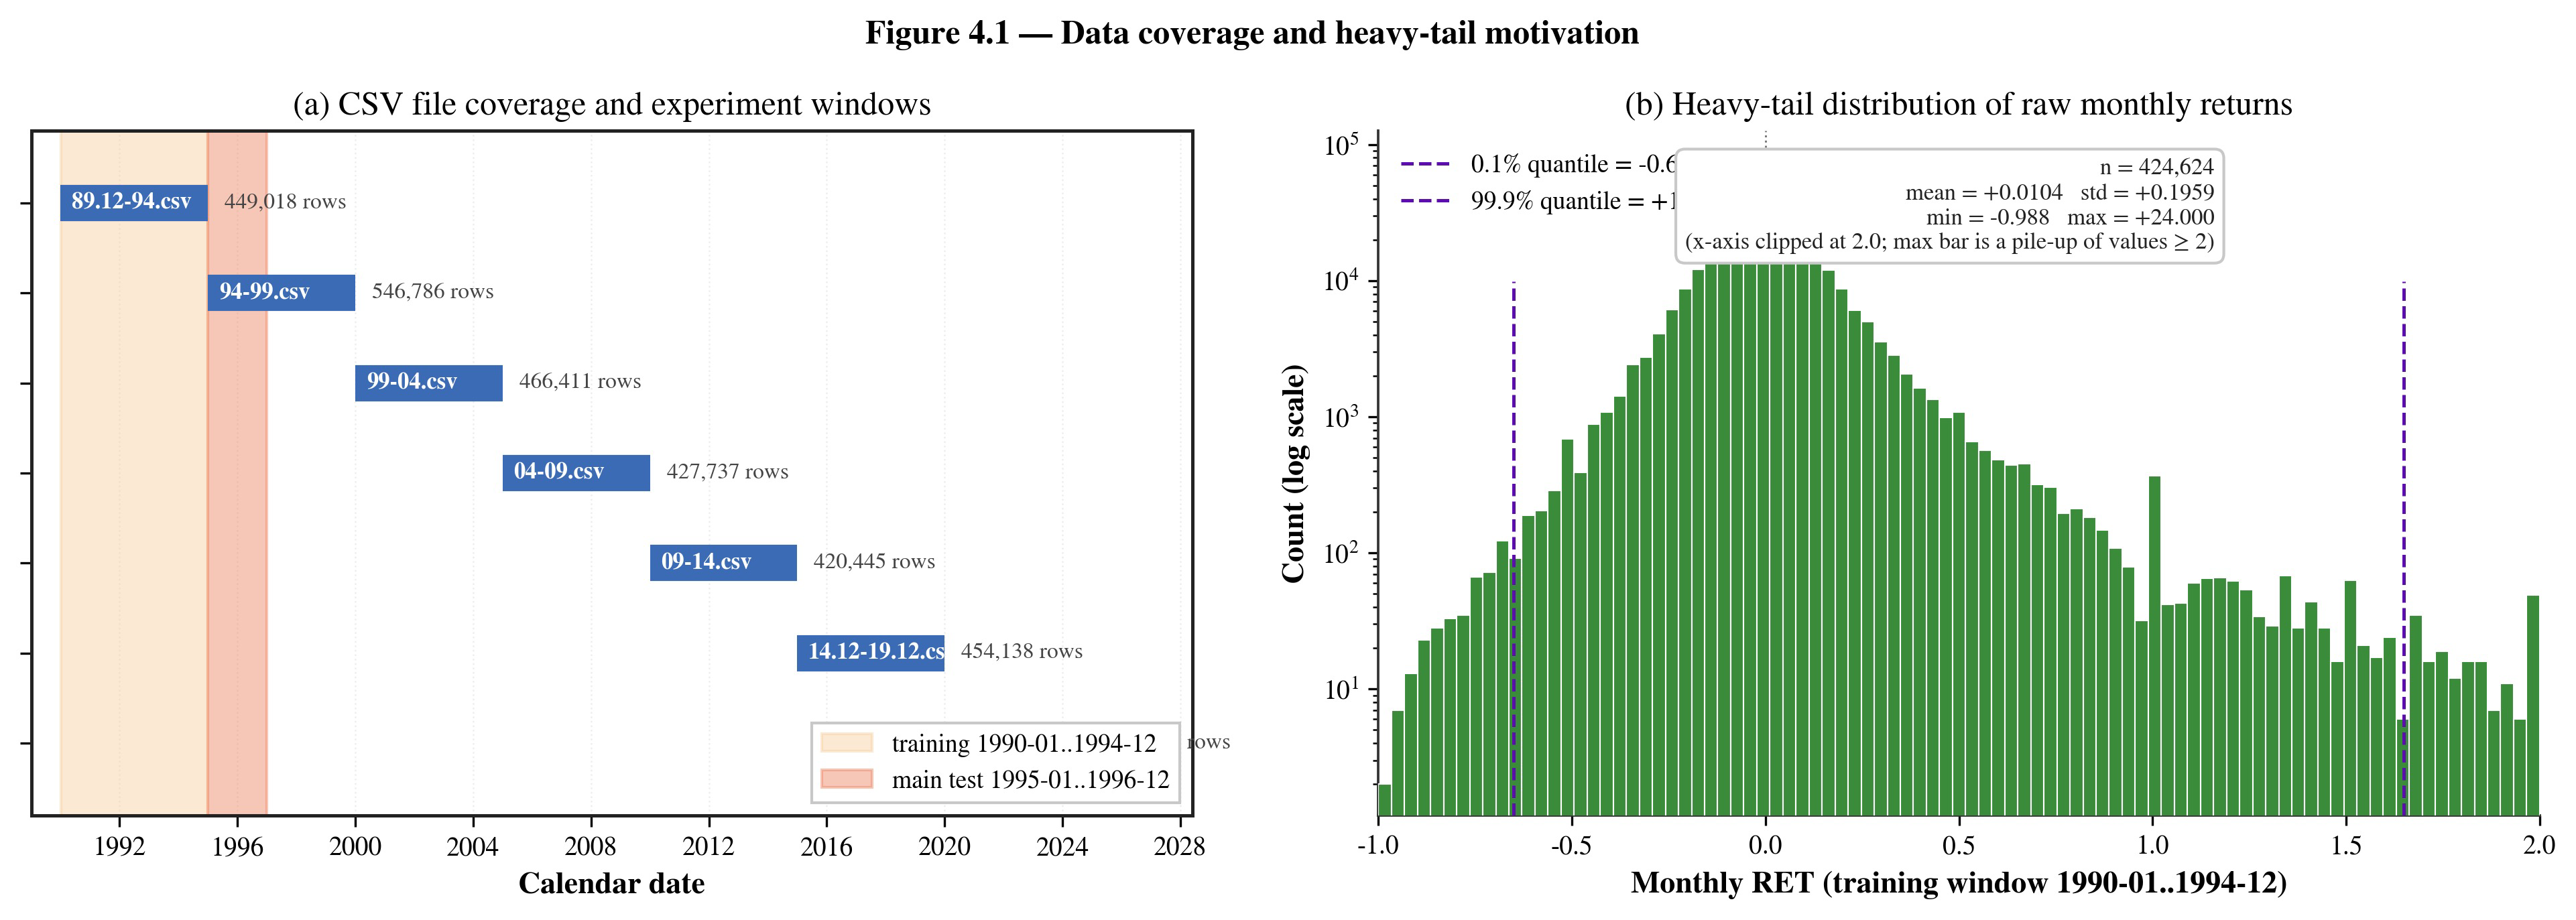
\includegraphics[width=0.9\textwidth]{figures/fig4_1_data_coverage.png}
\caption[Data coverage and training-era return distribution]{Data coverage and training-era return distribution.}
\label{fig:data-coverage}
\end{figure}

\section{Sample construction}\label{sec:sample-construction}

Three derived variables are computed on the raw panel before any feature set is built:

\begin{enumerate}
 \item Simple return $r_{i,t}$ is a numeric copy of \texttt{RET}, with any non-numeric entries coerced to \texttt{NaN} and dropped downstream.
 \item Monthly turnover is
 \[
 \text{to}_{i,t} = \frac{\text{VOL}_{i,t}}{\text{SHROUT}_{i,t} \times 1000},
 \]
 with zero-denominator rows set to \texttt{NaN} and infinities replaced by \texttt{NaN}. The factor of $1000$ converts shares-outstanding from CRSP's thousand-share unit into absolute shares, so \texttt{to} is a dimensionless volume-to-float ratio.
 \item The prediction target is the one-month-ahead return of the same security,
 \[
 y_{i,t} = r_{i,t+1},
 \]
 computed by a within-\texttt{PERMNO} one-step forward shift. Rows with missing $y_{i,t}$ are dropped. This definition prevents look-ahead leakage because features at time $t$ are constructed from information known at or before $t$ (see \S\ref{sec:feature-variables}) while $y_{i,t}$ only uses the realised return at $t+1$, provided that feature rows are built only from lagged variables as described in \S\ref{sec:feature-variables}.
\end{enumerate}

After these steps, any row missing any of \texttt{\{r, to, target\_ret\}} is dropped. The resulting panel is what every loss function consumes during training and evaluation.

\section{Train/test split}\label{sec:train-test-split}

The report uses a single static split, not a rolling or expanding-window scheme. The split is:

\begin{table}[H]
\centering
\caption{Static train/test split.}\label{tab:train-test-split}
\begin{tabular}{ccccc}\toprule
Partition & Start & End & Months & Role \\\midrule
Training & \texttt{1990-01} & \texttt{1994-12} & 60 & fit loss and compute gradients \\
Test (main) & \texttt{1995-01} & \texttt{1996-12} & 24 & out-of-sample evaluation for every final headline table \\
\bottomrule
\end{tabular}
\end{table}

The split is defined by date, not by security. A given \texttt{PERMNO} can contribute to both the training and test partitions; the prohibition on leakage is enforced at the time dimension via the shift in \S\ref{sec:sample-construction} and via the strict month cutoff above. No retraining occurs during the test window; the test period is a held-out evaluation of a single model per loss and per seed.

Chapter~5 labels every final headline number with the exact window start and end. Every final verification JSON confirms \texttt{row\_count = 24}, \texttt{first\_month = 1995-01}, and \texttt{last\_month = 1996-12} for the baseline and Phase~2 tables (see Appendix~B \S B.5). The multi-seed Phase~3 runs inherit the same window.

\section{Feature variables}\label{sec:feature-variables}

The repository implements multiple feature sets. The final report uses feature set \textbf{X1} throughout; alternative feature sets were not carried into the final empirical tables.

\subsection{X1 --- cumulative return and cumulative turnover (used throughout)}\label{subsec:x1}

The X1 feature set contributes 10 engineered columns (5 horizons $\times$ 2 variables), following the cumulative-return and cumulative-turnover construction of Medhat and Schmeling (2021) \cite{ref11} and Daniel and Moskowitz (2016) \cite{ref3}. The model input is 15 columns comprising these 10 X1 columns together with the 5 base panel columns (RET, VOL, SHROUT, r, to) that \texttt{assemble\_feature\_matrix} retains.

Formally, with $r_{i,t-1}$ denoting the one-month-lagged simple return (to avoid look-ahead for the $t+1$ target) and $\text{to}_{i,t-1}$ the one-month-lagged turnover:

\begin{itemize}
 \item Cumulative return over $w$ months:
 \[
 \mathrm{cr}^{(w)}_{i,t} = \prod_{k=1}^{w} \big(1 + r_{i,t-k}\big) - 1.
 \]
 \item Cumulative turnover over $w$ months:
 \[
 \mathrm{co}^{(w)}_{i,t} = \sum_{k=1}^{w} \text{to}_{i,t-k}.
 \]
\end{itemize}

Both aggregations require the full rolling window (\texttt{min\_periods = window}); rows for which any of the 15 columns is \texttt{NaN} are dropped. This is why the effective training sample begins roughly twelve months after the raw start date: the panel truncates naturally at the longest lookback.

The complete 15-column model input is listed in Appendix~B Table~B.3.

X1 is the feature set used in every run that produces a Chapter~5 number. The shared model configuration (\texttt{input\_dim}: 15, \texttt{hidden\_dims}: [64, 32, 16], \texttt{activation}: ReLU, \texttt{dropout}: 0.2) matches this feature width exactly.

Alternative feature-set constructors exist in the codebase but were not run under the final 24-month protocol. Feature-set sensitivity is therefore excluded from the main report and listed as future work in Chapter~6.

\section{Preprocessing}\label{sec:preprocessing}

The end-to-end preprocessing pipeline executes the following steps in order, on the concatenated raw panel:

\begin{enumerate}
 \item \textbf{Date parsing.} \texttt{date} is coerced to pandas \texttt{datetime}; any unparsable value raises an error, forcing the caller to confront malformed input rather than silently drop rows.
 \item \textbf{Column validation.} The loader checks that \texttt{\{PERMNO, date, RET, VOL, SHROUT\}} are present. Missing columns raise a \texttt{KeyError} before any numeric work runs.
 \item \textbf{Missing-value filling.} Within each \texttt{PERMNO}, \texttt{\{RET, VOL, SHROUT\}} are forward-filled (default \texttt{method='ffill'}). This treats a missing observation as the continuation of the last observed value for that security. Forward-filling returns can fabricate an observation for a genuinely inactive name-month; this is an implementation choice rather than a universally conservative treatment, and is noted as a data limitation in \S\ref{sec:data-limitations}. Any row that remains \texttt{NaN} after the fill is dropped.
 \item \textbf{Basic-variable construction.} Numeric \texttt{r} and \texttt{to} are computed as described in \S\ref{sec:sample-construction}. Any $\pm\infty$ produced by zero-share-outstanding rows is replaced by \texttt{NaN}.
 \item \textbf{Target construction.} \texttt{target\_ret = r.shift(-1)} within each \texttt{PERMNO}. Rows without a valid \texttt{target\_ret} are dropped.
 \item \textbf{Row-level completeness filter.} Any row still missing any of \texttt{\{r, to, target\_ret\}} is dropped.
\end{enumerate}

At the feature-building stage, each \texttt{build\_feature\_set\_xN} function additionally drops rows whose feature columns contain any \texttt{NaN}. For X1 this cascades through every 1-, 3-, 6-, 9-, and 12-month lookback window.

Two aspects are deliberately \emph{not} applied by the pipeline and are worth stating explicitly:

\begin{itemize}
 \item \textbf{No winsorisation.} The raw \texttt{RET} distribution has extreme tails (training-era maximum of $+2400\%$ for a single name-month). The pipeline does not clip or winsorise the return series. Heavy tails are the motivation for robust-loss design; normalising them away at the data stage would obscure the effect the loss functions are intended to handle. Chapter~3 discusses how each loss family treats these outliers mathematically. Because the 15 model inputs include raw RET, VOL, SHROUT, r, and to (Appendix~B Table~B.3), extreme values in these base columns enter the MLP directly.
 \item \textbf{No cross-sectional clipping of predictions.} Any clipping is performed inside the portfolio construction module (Chapter~3 \S3.5) on prediction $z$-scores, not on input features. Input features are used as-is.
\end{itemize}

\section{Data limitations}\label{sec:data-limitations}

Several limitations of the data scope the empirical claims of this report:

\begin{enumerate}
 \item \textbf{Single market and single frequency.} The panel is US-listed equities at monthly frequency. Results do not generalise directly to higher frequencies (daily, intraday), other asset classes, or non-US markets. Any extension of the loss-design conclusions to those regimes requires re-estimation.
 \item \textbf{Single evaluation window.} The main test window is fixed at 1995-01 to 1996-12. Macroeconomic regime effects are not sampled; in particular, the window spans a sustained bull market and does not include the 1997--98 crises, the 2000 tech correction, or the 2008 financial crisis. Robustness across regimes is listed as future work in Chapter~6.
 \item \textbf{Heavy-tailed returns.} As quoted in \S\ref{sec:data-source}, the training-era \texttt{RET} series includes name-months with returns exceeding $+1000\%$. Such extremes dominate any scale-sensitive quantity (MSE, R$^{2}$) and drive the divergent R$^{2}$ values observed in Chapter~5. Readers should interpret R$^{2}$ as a diagnostic rather than a primary performance metric in this setting.
 \item \textbf{Sample coverage changes over time.} The training window contains 10,987 unique \texttt{PERMNO}s; the source file covers 61 month-sections. The panel grows substantially in later files (for example, 94-99.csv contains 12,836 unique \texttt{PERMNO}s). The Phase~2 multi-seed runs still use the 1990--1996 window, so this sample-growth effect does not bias the comparison; however, any rolling-window extension would need to account for sample composition drift.
 \item \textbf{No survivorship-bias correction.} The pipeline does not filter delisted securities or adjust for delisting returns. CRSP monthly files typically include delisting rows via \texttt{RET}, but bias from partial delisting data has not been verified. Long-short performance can be biased materially by missing delisting returns, particularly in the short leg where delistings cluster. Conclusions drawn from long-short Sharpe should be read with this implicit assumption in mind.
 \item \textbf{Feature-set restriction.} All Chapter~5 evidence uses X1. Feature sensitivity is untested because alternative feature sets were not run under the final protocol.
\end{enumerate}

These limitations are revisited in Chapter~6 together with the methodological limitations of the static-window protocol.

\cleardoublepage

\chapter{Empirical Results and Discussion}

\label{ch:empirical-results-and-discussion}

This chapter reports the empirical performance of every loss function that enters the final recommendation. All numbers quoted here are traceable to a single source-of-truth evidence map; each caption records the evaluation window, the seed set, and the underlying artifact path so the reader can audit the claim.

The structure of the chapter mirrors the empirical pipeline rather than the order in which the experiments were carried out. Section~5.1 restates the shared evaluation protocol. Sections~5.2--5.3 present same-window single-seed comparisons (baseline losses and the hybrid A/M sweep, both at seed 42); within each comparison table, the loss function is the only varying factor. Sections~5.4--5.5 move to multi-seed evidence on the M2-robust family and the broader $\alpha/\beta/\lambda$ sweeps, which form the basis of the final recommendation; cross-phase comparisons differ in additional dimensions (\S5.7). Section~5.6 discusses a loss-component normalisation probe. Section~5.7 scopes the boundary of cross-phase comparison claims. Section~5.8 synthesises the headline findings and bridges to the conclusion.

\section{Evaluation protocol recap}

\label{sec:evaluation-protocol-recap}

All experiments use the protocol defined in Chapter~3 \S3.4 and the X1 feature input from Chapter~4. The key operational parameters are: train \texttt{1990-01..1994-12} (60 months), test \texttt{1995-01..1996-12} (24 months), MLP[64,32,16]+ReLU+dropout 0.2, batch size 1024, 20 epochs, top/bottom 10\% signal-tilted long-short portfolio with 5\% per-name cap. Sharpe is annualised as $\sqrt{12} \cdot \bar r / \sigma_r$. Single-seed tables (\S5.2--\S5.3) use seed 42; multi-seed tables (\S5.4--\S5.6) use three seeds per row. Source paths are listed in each table caption; full reproduction commands are in Appendix~B.

\section{Phase 1: Baseline loss comparison (24 months, seed 42)}

\label{sec:phase1-baseline-loss-comparison}

Table~\ref{tab:baseline-loss-comparison} reports the main baseline-loss comparison under the static 24-month window at seed 42. The seven rows cover the traditional regression losses (MSE, MedSE), the absolute-loss family (MADL, GMADL, IMADL), and the two hybrid multiplicative variants (\texttt{hybrid\_mul\_m1}, \texttt{hybrid\_mul\_m2}) that will be extended in \S5.3.

\begin{table}[H]
\centering
\caption{Baseline loss comparison. Static train \texttt{1990-01..1994-12}, test \texttt{1995-01..1996-12}, seed 42, MLP[64,32,16]+ReLU+dropout 0.2, X1, batch 1024, 20 epochs, top/bottom 10\% with 5\% per-name cap. Source: see Appendix~B \SB.4.}
\label{tab:baseline-loss-comparison}
\begin{tabular}{cccccc}
\toprule
Loss & Sharpe & Cum.\ return & Avg R$^2$ & Avg monthly LS & Monthly LS std \\
\midrule
MSE & $-0.4643$ & $-0.1125$ & $-102.1787$ & $-0.004422$ & $0.032989$ \\
MedSE & $0.0932$ & $0.0060$ & $-2\,297\,042.29$ & $0.001214$ & $0.045124$ \\
MADL & $-0.3058$ & $-0.0756$ & $-4.15 \times 10^{9}$ & $-0.002794$ & $0.031653$ \\
GMADL & $0.2025$ & $0.0279$ & $-7.02 \times 10^{9}$ & $0.001429$ & $0.024449$ \\
IMADL & $-0.3732$ & $-0.0944$ & $-106.5114$ & $-0.003578$ & $0.033211$ \\
\texttt{hybrid\_mul\_m1} & $0.4435$ & $0.0509$ & $-4.7942$ & $0.002215$ & $0.017302$ \\
\texttt{hybrid\_mul\_m2} & $-0.0017$ & $-0.0032$ & $-1.0298$ & $-0.000008$ & $0.016096$ \\
\bottomrule
\end{tabular}
\end{table}

Three observations follow from the table.

First, neither traditional regression loss yields an economically meaningful long-short portfolio at this single seed. MSE is strongly negative in both Sharpe and cumulative return, and MedSE is only nominally positive (Sharpe $0.0932$, cumulative return $+0.60\%$ over 24 months). This stands in contrast to earlier preliminary six-month checks in which MedSE appeared to dominate; under the same protocol extended to 24 months at seed 42, the MedSE advantage vanishes and the headline numbers belong in \S5.4 to the multi-seed M2-robust family, not to MedSE.

Second, the absolute-loss family produces extremely negative average R$^2$ values ($-4.15 \times 10^{9}$ for MADL and $-7.02 \times 10^{9}$ for GMADL). This does not indicate that the portfolio signal is uninformative -- GMADL yields a positive Sharpe ($0.2025$), second among the non-hybrid baselines (behind only \texttt{hybrid\_mul\_m1}). Rather, the point-prediction scale has diverged from the realised-return scale: under a direction/magnitude-weighted objective the MLP produces predictions that are orders of magnitude away from the realised return in absolute terms. Because the long-short construction uses only the cross-sectional rank of the predictions, portfolio performance is decoupled from calibration quality. This decoupling is central to interpreting the rest of the chapter: absolute-loss-style variants should be evaluated by their ranked portfolio metrics (Sharpe, cumulative return) and, where multi-seed evidence exists, CV across seeds, rather than by R$^2$.

Third, among baseline losses, \texttt{hybrid\_mul\_m1} yields the best single-seed Sharpe at $0.4435$, nearly twice the next-highest. Its cumulative return over 24 months is $+5.09\%$ and its monthly LS standard deviation is the lowest of the set at $0.017302$, suggesting that combining a directional-prediction term with a rank-preserving term produces a more stable long-short signal than either an MSE or an MADL-style term alone. This result motivates the hybrid sweep in \S5.3.

Table~\ref{tab:baseline-loss-comparison} is a same-window single-seed comparison. It is informative for ranking loss families at a fixed seed but cannot support statements about robustness to seed perturbation. Seed-sensitivity claims are reserved for \S5.4 and \S5.5.

\begin{figure}[H]
\centering
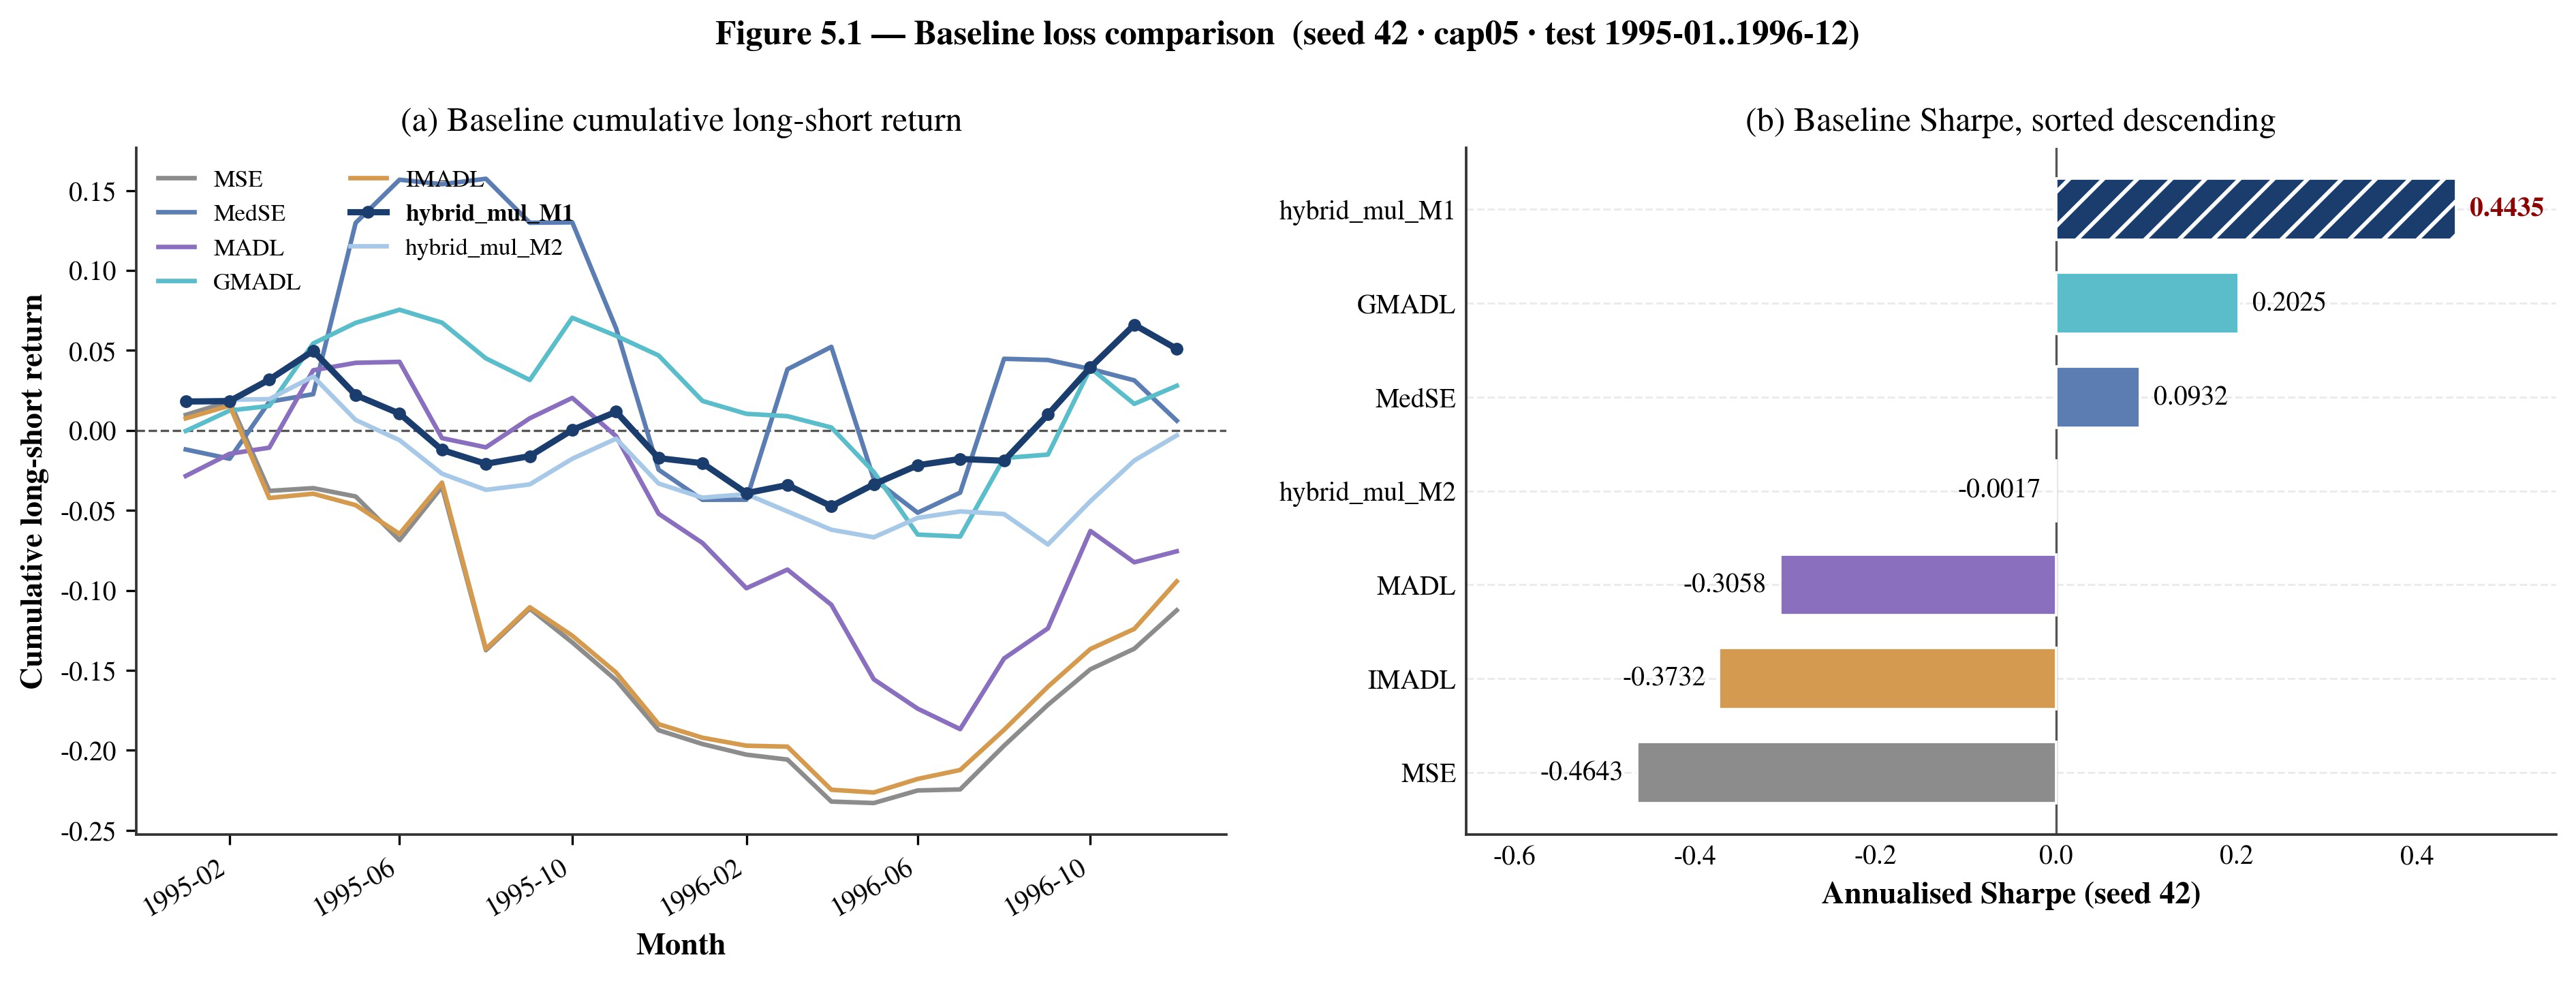
\includegraphics[width=0.9\textwidth]{figures/fig5_1_baseline_comparison.png}
\caption[Baseline loss comparison: cumulative return and Sharpe]{Baseline loss comparison. Left: monthly cumulative long-short return per loss over 1995-01..1996-12; \texttt{hybrid\_mul\_m1} is drawn bold with markers. Right: annualised Sharpe sorted descending, with \texttt{hybrid\_mul\_m1} hatched in deep navy as the seed-42 peak. Seed 42, cap05 portfolio, MLP[64,32,16]+ReLU+dropout 0.2, X1, batch 1024, 20 epochs.}
\label{fig:baseline-loss-comparison}
\end{figure}

\section{Phase 2: Hybrid A/M variant sweep (24 months, seed 42)}

\label{sec:phase2-hybrid-am-sweep}

This phase extends the two hybrid multiplicative variants of \S5.2 into a parameterised family of nine variants (additive A1--A5 and multiplicative M1--M4; see Chapter~3 \S3.3 for definitions). All nine runs use the same static window, feature set, and portfolio construction as Table~\ref{tab:baseline-loss-comparison}; only the loss specification changes.

\begin{table}[H]
\centering
\caption{Phase 2 additive (A1--A5) and multiplicative (M1--M4) variants. Static train \texttt{1990-01..1994-12}, test \texttt{1995-01..1996-12}, seed 42, same model / feature / portfolio configuration as Table~\ref{tab:baseline-loss-comparison}. Source: see Appendix~B \SB.4.}
\label{tab:phase2-variants}
\begin{tabular}{ccccc}
\toprule
Variant & Loss ID & Sharpe & Cum.\ return & Avg R$^2$ \\
\midrule
A1 & \texttt{hybrid\_add\_a1} & $0.1241$ & $0.0133$ & $-2\,105.95$ \\
A2 & \texttt{hybrid\_add\_a2} & $0.2173$ & $0.0450$ & $-484.75$ \\
A3 & \texttt{hybrid\_add\_a3} & $\mathbf{0.5738}$ & $\mathbf{0.0813}$ & $-1\,383.64$ \\
A4 & \texttt{hybrid\_add\_a4} & $0.2311$ & $0.0463$ & $-11\,229.79$ \\
A5 & \texttt{hybrid\_add\_a5} & $-0.4110$ & $-0.2080$ & $-507\,162.38$ \\
M1 & \texttt{hybrid\_mul\_m1} & $\mathbf{0.4435}$ & $\mathbf{0.0509}$ & $-4.79$ \\
M2 & \texttt{hybrid\_mul\_m2} & $-0.0017$ & $-0.0032$ & $-1.03$ \\
M3 & \texttt{hybrid\_mul\_m3} & $-0.9691$ & $-0.0903$ & $-0.44$ \\
M4 & \texttt{hybrid\_mul\_m4} & $-0.3440$ & $-0.0409$ & $-0.06$ \\
\bottomrule
\end{tabular}
\end{table}

The additive family peaks at A3 with Sharpe $0.5738$ and cumulative return $+8.13\%$; A4 and A2 are second-tier; A5 collapses as the added term overwhelms the base MSE contribution. The multiplicative family peaks at M1 with Sharpe $0.4435$ (identical to its Table~\ref{tab:baseline-loss-comparison} row because the runner and configuration are unchanged); M2 through M4 degrade monotonically on Sharpe.

A few interpretive notes matter for later sections. (i)~At seed 42, A3 slightly outperforms M1 on Sharpe and cumulative return, yet the multiplicative family is the one that Phase 3 extends into the M2-robust $\gamma$ parameterisation. The rationale for that design choice is discussed in Chapter~3; the empirical support is that A3's R$^2$ magnitude ($-1\,383.64$, driven by the additive MSE term being dominated by a scale-insensitive accuracy term) offers less interpretable control than the M-family, whose R$^2$ remains within a small single-digit range. (ii)~Seed-42 peaks do not survive seed perturbation uniformly. In \S5.4 the M2-robust $\gamma$ sweep is evaluated across three seeds and the ordering of mean Sharpe does not match the single-seed ordering in this table. Consequently, the Phase~1.5 rows should be read as \emph{motivation} for the Phase~2 design, not as a final variant ranking.

The additive family is not carried further into multi-seed robustness in this report. The final recommendation in \S5.8 draws on the multi-seed evidence for the M2-robust family (\S5.4) and on the integrated cross-variant sweep (\S5.5).

\begin{figure}[H]
\centering
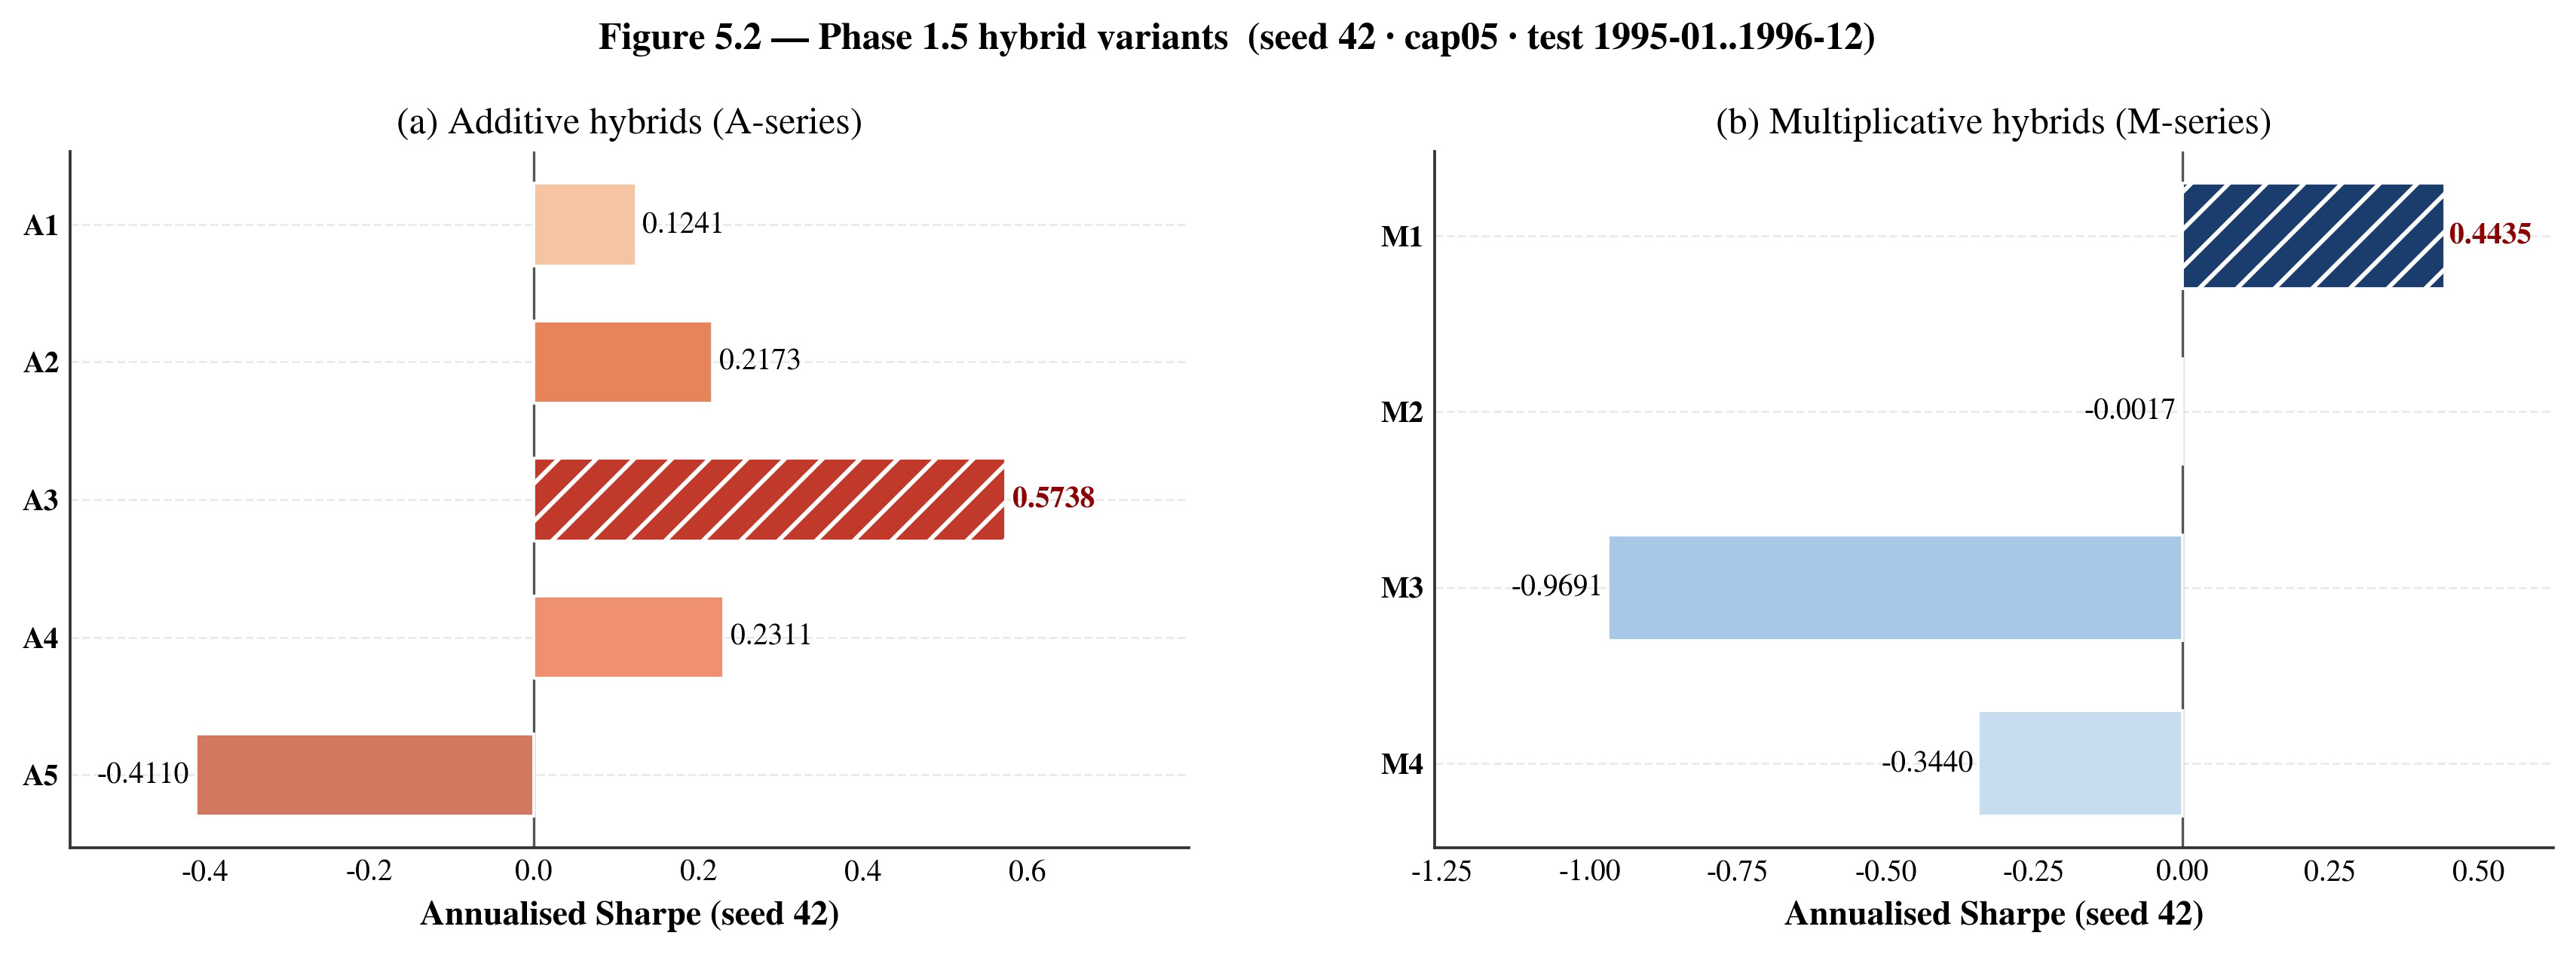
\includegraphics[width=0.9\textwidth]{figures/fig5_2_phase15_variants.png}
\caption[Phase 2 hybrid variants: additive A1--A5 and multiplicative M1--M4]{Phase 2 hybrid variants. Horizontal grouped bars showing annualised Sharpe for (a) additive A1--A5 (warm palette) and (b) multiplicative M1--M4 (cool palette); seed-42 peaks A3 and M1 are hatched in deep red/navy and their Sharpe values are rendered in dark-red bold. Same runner/feature/portfolio/architecture as Table~\ref{tab:baseline-loss-comparison}.}
\label{fig:phase2-variants}
\end{figure}

\section{Phase 3a: Multi-seed $\gamma$ refinement}

\label{sec:phase3a-gamma-refinement}

Phase~2 introduces an explicit robustness parameter $\gamma$ into the multiplicative hybrid M2 variant, producing the family of \texttt{m2\_robust\_gamma\{0.03, 0.05, 0.07, 0.10, 0.15\}} losses. Each variant is run across three random seeds using the same 24-month static window and the 5\% per-name portfolio cap (\texttt{cap05}). The purpose is to decouple the seed-42 ranking of \S5.3 from a claim about the expected performance of the loss under seed perturbation.

Sharpe stability is reported as the coefficient of variation $\mathrm{CV} = \sigma_S / |\mu_S|$, where $\mu_S$ and $\sigma_S$ are the cross-seed mean and standard deviation of the annualised Sharpe (same $\sqrt{12}$-annualised convention as \S5.1 and \S5.2). Lower CV implies lower relative seed sensitivity.

\begin{table}[H]
\centering
\caption{Phase 3a $\gamma$ refinement, multi-seed (3 seeds per row). Static train \texttt{1990-01..1994-12}, test \texttt{1995-01..1996-12}, \texttt{cap05} portfolio cap. Each row aggregates three seeds. Source: see Appendix~B \SB.4.}
\label{tab:gamma-refinement}
\begin{tabular}{cccccc}
\toprule
Loss & Runs & Sharpe mean & Sharpe std & Cum.\ return mean & CV \\
\midrule
\texttt{m2\_robust\_gamma03} & 3 & $0.3234$ & $0.3418$ & $0.0818$ & $1.0570$ \\
\texttt{m2\_robust\_gamma05} & 3 & $0.7054$ & $0.1488$ & $0.2392$ & $0.2109$ \\
\texttt{m2\_robust\_gamma07} & 3 & $\mathbf{0.9156}$ & $0.1655$ & $\mathbf{0.2799}$ & $\mathbf{0.1808}$ \\
\texttt{m2\_robust\_gamma10} & 3 & $1.0043$ & $0.5638$ & $0.2368$ & $0.5613$ \\
\texttt{m2\_robust\_gamma15} & 3 & $0.8163$ & $0.3724$ & $0.2277$ & $0.4562$ \\
\bottomrule
\end{tabular}
\end{table}

\vspace{-1em}
\begin{figure}[H]
\centering

\includegraphics[width=0.9\textwidth]{figures/fig5_3_gamma_refinement.png}
\caption[Phase 3a $\gamma$ refinement: multi-seed Sharpe and stability]{Phase 3a $\gamma$ refinement: multi-seed Sharpe and stability. Left: cross-seed mean annualised Sharpe with $\pm 1$ std error bars (3 seeds per $\gamma$); light vertical bars indicate the min--max range. Right: coefficient of variation CV $= \sigma / |\mu|$. Evaluation window \texttt{1995-01..1996-12}, \texttt{cap05} portfolio cap.}
\label{fig:gamma-refinement}
\end{figure}

Figure~\ref{fig:gamma-tuning-curve} presents the same $\gamma$ sweep as a continuous tuning curve, adding a third panel that reports the mean monthly long-short return standard deviation across seeds. The three-panel view makes the trade-off explicit: \texttt{gamma07} sits at the stability peak on all three dimensions simultaneously -- it does not merely minimise CV while sacrificing Sharpe, nor does it minimise portfolio volatility at the cost of return. \texttt{gamma10} is visibly higher on the Sharpe axis but also higher on both the CV and the volatility axes, confirming that its apparent Sharpe advantage comes with a measurable increase in prediction-level variance.

\begin{figure}[H]
\centering
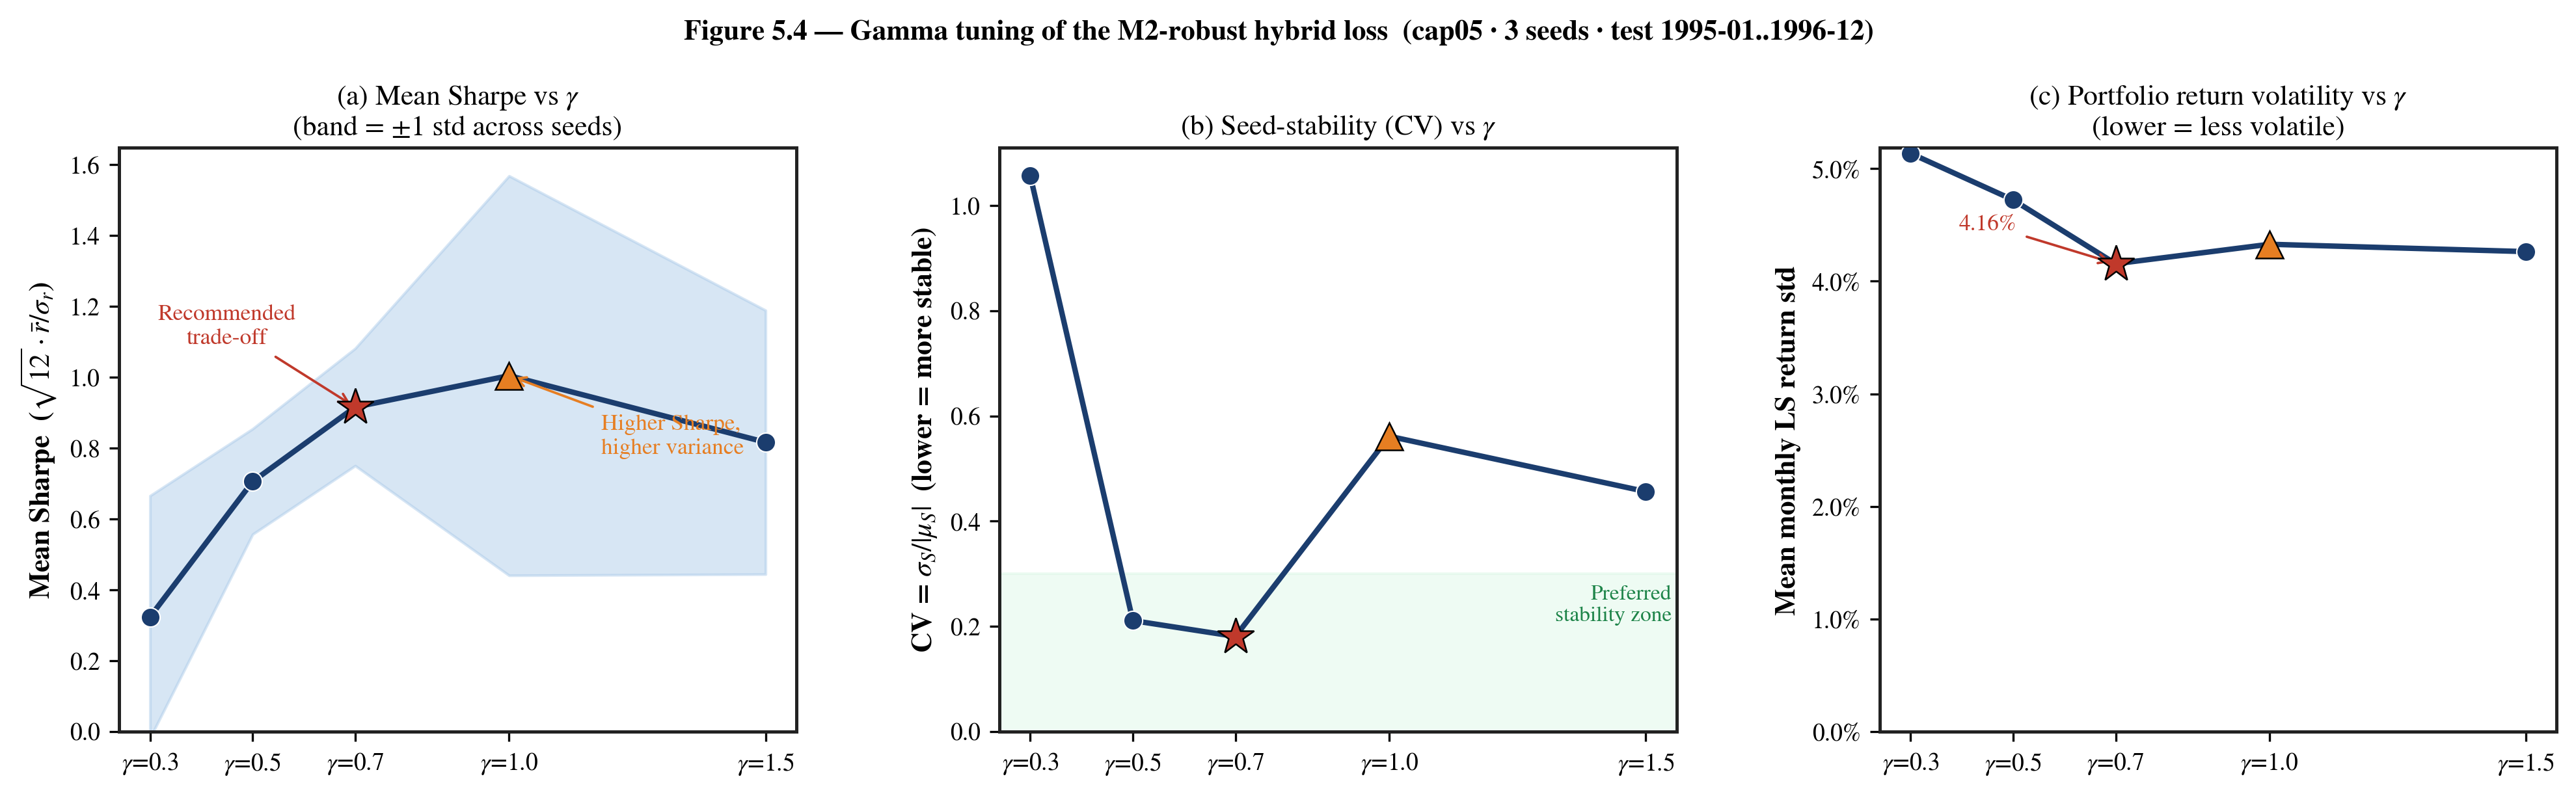
\includegraphics[width=0.9\textwidth]{figures/fig5_4_gamma_tuning_curve.png}
\caption[$\gamma$ tuning curve: Sharpe, stability, and portfolio volatility]{$\gamma$ tuning curve: Sharpe, stability, and portfolio volatility. Panel~(a): mean annualised Sharpe vs $\gamma$ with $\pm 1$ std band across 3 seeds. Panel~(b): cross-seed CV vs $\gamma$; green shading marks the preferred stability zone (CV $\leq 0.30$). Panel~(c): mean monthly long-short return standard deviation vs $\gamma$ -- a direct measure of portfolio-level variance. Red star: \texttt{gamma07} (recommended); orange triangle: \texttt{gamma10} (higher Sharpe, higher variance). Evaluation window \texttt{1995-01..1996-12}, \texttt{cap05}, 3 seeds per row.}
\label{fig:gamma-tuning-curve}
\end{figure}

Three findings follow from Table~\ref{tab:gamma-refinement}.

First, \texttt{m2\_robust\_gamma07} provides the best Sharpe-vs-stability trade-off in the $\gamma$ sweep. Its mean Sharpe of $0.9156$ is within $9\%$ of the highest mean ($1.0043$ for \texttt{gamma10}), while its coefficient of variation is the lowest among the non-collapsed variants at $0.1808$ -- roughly one-third of the CV of \texttt{gamma10}. Its mean cumulative return of $+27.99\%$ over 24 months is the largest in the table. Across three seeds, its minimum Sharpe is $0.7532$; no seed in the run produces a negative Sharpe.

Second, \texttt{m2\_robust\_gamma10} has the highest mean Sharpe ($1.0043$) but also the highest CV among the strong variants ($0.5613$). Its per-seed Sharpe range is wide ($0.4587$ to $1.5847$). Interpreted cautiously, \texttt{gamma10} is a variant whose \emph{best} seed produces the best Sharpe of the entire $\gamma$ family, but whose \emph{average} seed has not materially improved on \texttt{gamma07}. A recommendation that selects the variant with the highest mean Sharpe should therefore come with an explicit seed-sensitivity caveat.

Third, the $\gamma$ schedule exhibits a non-monotone relationship with Sharpe stability. \texttt{gamma03} collapses almost entirely (CV $1.0570$, minimum Sharpe negative), and \texttt{gamma15} -- past the stability peak -- also degrades sharply in CV ($0.4562$) even though its mean Sharpe remains respectable ($0.8163$). The stability peak near $\gamma = 0.07$ is thus an internal optimum of the robust component rather than the endpoint of a monotone trend. This is consistent with the design intent of the robust modifier: too little robustness under-weights the rank-preserving term; too much robustness flattens the loss surface and re-injects seed-level noise into the learned weights.

On this evidence alone, \texttt{m2\_robust\_gamma07} is the best-supported candidate for the primary recommendation in \S5.8. The fuller comparison in \S5.5 -- where \texttt{gamma07} is evaluated against $\alpha$- and $\beta$-sweep variants from other families -- confirms this ordering.

\section{Phase 3b: Integrated $\alpha$, $\beta$, and $\lambda$ sweeps}

\label{sec:phase3b-integrated-sweeps}

To rule out the possibility that the M2-robust $\gamma$ family is merely a locally good design in the hybrid-multiplicative corner of the loss space, Phase~2 also runs an integrated sweep over three other parameterised families: the IMADL-m2 $\alpha$ sweep, the IMADL-GMADL $\beta$ sweep, and an adaptive-$\lambda$ family. Table~\ref{tab:integrated-summary} reports selected grouped summaries; the complete table contains further fine-grained $\gamma$ variants (\texttt{gamma001}, \texttt{gamma01}) used for locating the $\gamma$ optimum. Note that \texttt{m2\_robust\_gamma07}, the primary recommendation, is reported in Table~\ref{tab:gamma-refinement} and serves as the reference line in Figure~\ref{fig:gamma-refinement}.

Source: integrated grouped summary CSV (see Appendix~B \SB.3 for the exact branch path). All rows are 3-seed averages at \texttt{cap05} with the same 24-month window as Table~\ref{tab:gamma-refinement}.

\begin{table}[H]
\centering
\caption{Phase 2 integrated summary across $\alpha$, $\beta$, $\lambda$ families (selected rows). Static train \texttt{1990-01..1994-12}, test \texttt{1995-01..1996-12}, \texttt{cap05}, 3 seeds per row.}
\label{tab:integrated-summary}
\begin{tabular}{ccccc}
\toprule
Loss & Sharpe mean & Sharpe std & Cum.\ return mean & CV \\
\midrule
\texttt{adaptive\_lambda10} & $0.4938$ & $0.7617$ & $0.0618$ & $1.5426$ \\
\texttt{adaptive\_lambda50} & $0.2763$ & $0.1597$ & $0.0817$ & $0.5780$ \\
\texttt{adaptive\_lambda100} & $0.0955$ & $0.0343$ & $0.0021$ & $0.3591$ \\
\texttt{imadl\_gmadl\_beta03} & $-0.0345$ & $0.1381$ & $-0.0424$ & $4.0084$ \\
\texttt{imadl\_gmadl\_beta05} & $0.0406$ & $0.4116$ & $-0.0138$ & $10.1328$ \\
\texttt{imadl\_gmadl\_beta07} & $-0.0020$ & $0.2747$ & $-0.0409$ & $139.51$ \\
\texttt{imadl\_m2\_alpha02} & $0.1788$ & $1.1576$ & $0.2225$ & $6.4735$ \\
\texttt{imadl\_m2\_alpha03} & $0.2159$ & $0.2010$ & $0.0588$ & $0.9310$ \\
\texttt{imadl\_m2\_alpha04} & $0.3540$ & $0.0656$ & $0.0962$ & $0.1853$ \\
\texttt{imadl\_m2\_alpha05} & $0.5822$ & $0.3193$ & $0.2465$ & $0.5484$ \\
\texttt{imadl\_m2\_alpha06} & $\mathbf{0.6895}$ & $0.1685$ & $\mathbf{0.3042}$ & $\mathbf{0.2443}$ \\
\texttt{imadl\_m2\_alpha07} & $0.4024$ & $0.2466$ & $0.1036$ & $0.6128$ \\
\texttt{imadl\_m2\_alpha08} & $0.5683$ & $0.4130$ & $0.2071$ & $0.7267$ \\
\texttt{m2\_robust\_gamma001} & $0.6919$ & $0.8258$ & $0.1705$ & $1.1936$ \\
\texttt{m2\_robust\_gamma01} & $0.7470$ & $0.3937$ & $0.2718$ & $0.5270$ \\
\texttt{m2\_robust\_gamma10} & $1.0043$ & $0.5638$ & $0.2368$ & $0.5613$ \\
\bottomrule
\end{tabular}
\end{table}

\begin{figure}[H]
\centering

\includegraphics[width=0.9\textwidth]{figures/fig5_5_imadl_alpha_sweep.png}
\caption[IMADL-m2 $\alpha$ sweep vs $\gamma$ reference]{IMADL-m2 $\alpha$ sweep vs $\gamma$ reference. Left: cross-seed mean annualised Sharpe with $\pm 1$ std error bars for $\alpha \in \{0.2, \ldots, 0.8\}$; dashed horizontal lines mark the mean Sharpe of \texttt{m2\_robust\_gamma07} (red) and \texttt{m2\_robust\_gamma10} (orange) as references. Right: coefficient of variation on a log scale, with the same $\gamma$ references. Evaluation window \texttt{1995-01..1996-12}, \texttt{cap05}, 3 seeds per row. Source: integrated grouped summary CSV and $\gamma$ refinement grouped summary (see Appendix~B \SB.3 for exact paths).}
\label{fig:imadl-alpha-sweep}
\end{figure}

The IMADL-m2 $\alpha$ sweep produces a clean unimodal Sharpe curve with a peak at \texttt{alpha06} (mean Sharpe $0.6895$, cumulative return $+30.42\%$, CV $0.2443$). Below the peak, \texttt{alpha04} and \texttt{alpha05} remain competitive and, in the case of \texttt{alpha04}, even more stable (CV $0.1853$) at the cost of substantially lower mean Sharpe. Above the peak, \texttt{alpha07} and \texttt{alpha08} degrade. The peak's mean Sharpe is below the \texttt{gamma07} mean but its cumulative return is slightly higher, and its seed-sensitivity is only moderately worse. IMADL-m2 $\alpha$06 is therefore a sensible fallback for interpretations that prioritise cumulative return over volatility.

The IMADL-GMADL $\beta$ family does not produce a robust positive Sharpe across seeds. All three $\beta$ values have mean Sharpe close to zero and CV values in the single digits or larger ($\beta$07 has CV $\sim 140$, arising from a near-zero mean Sharpe). This indicates that directly composing IMADL with the GMADL exponent introduces scale instabilities similar to those observed in \S5.2 for GMADL alone, and normal $\beta$-tuning does not recover the stability of \texttt{m2\_robust\_gamma07}. No $\beta$ row is carried into the final recommendation.

The adaptive-$\lambda$ family, in which the relative weighting of the robust and directional terms is tuned during training, underperforms both in mean Sharpe and in stability. The best row in the family (\texttt{adaptive\_lambda10}) has mean Sharpe $0.4938$ but CV $1.5426$ -- the largest among the non-IMADL-m2-$\alpha$02 and non-GMADL-$\beta$ rows in Table~\ref{tab:integrated-summary} (only \texttt{imadl\_m2\_alpha02} at CV $6.4735$ and the $\beta$ family exceed it). The ordering $\lambda$10 $>$ $\lambda$50 $>$ $\lambda$100 indicates the family prefers moderate weighting, but even the best moderate setting does not reach the $\gamma$ or $\alpha$ peaks.

Combining Table~\ref{tab:gamma-refinement} and Table~\ref{tab:integrated-summary} confirms that the two best candidates in the final recommendation come from the two self-consistent peaks: \texttt{m2\_robust\_gamma07} at Sharpe $0.9156$ / CV $0.1808$, and \texttt{imadl\_m2\_alpha06} at Sharpe $0.6895$ / CV $0.2443$.

Figure~\ref{fig:sharpe-cv-frontier} places all multi-seed hybrid variants on a single Sharpe-stability plane, making the frontier structure visible. The preferred region -- high Sharpe, low CV -- is occupied exclusively by \texttt{gamma07}. \texttt{gamma10} lies outside the preferred region on the CV axis despite its higher mean Sharpe. \texttt{alpha06} lies inside the preferred region on the CV axis but below \texttt{gamma07} on the Sharpe axis. No other variant from the $\alpha$, $\beta$, or adaptive-$\lambda$ families reaches the preferred region. The frontier view confirms that the recommendation is not a local optimum within a single family but the dominant point across the full hybrid design space explored in this study.

\begin{figure}[H]
\centering
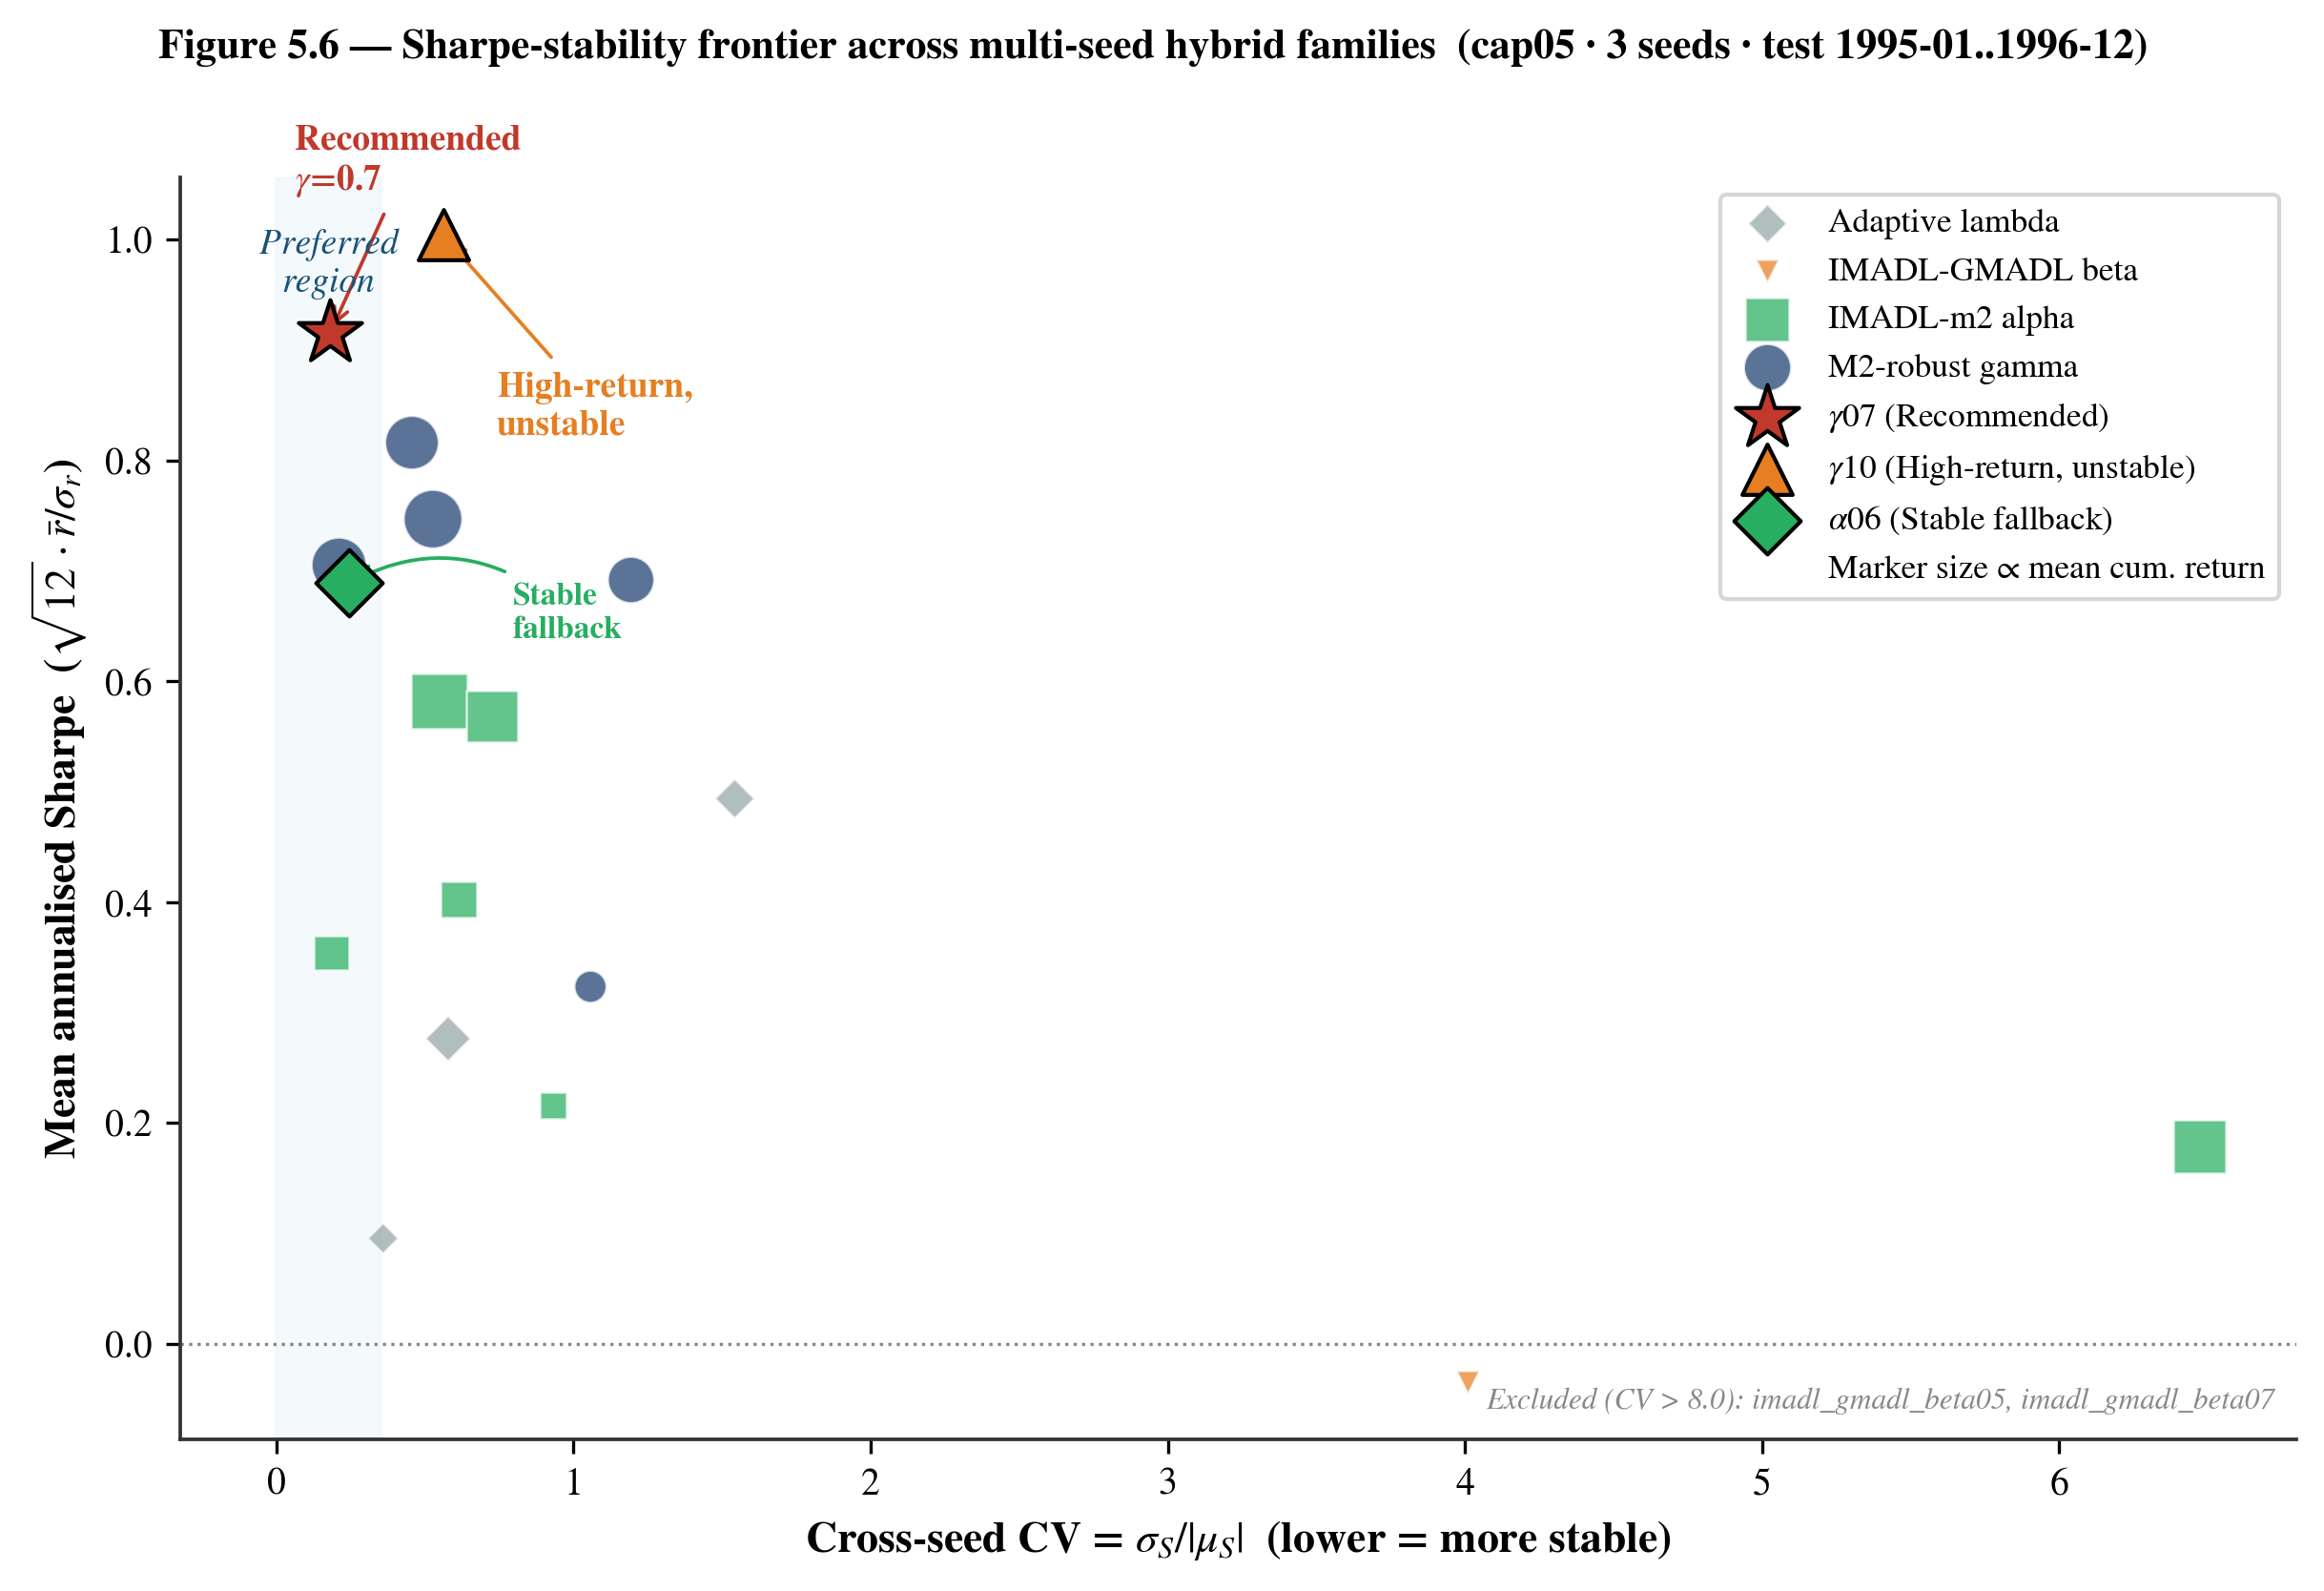
\includegraphics[width=0.9\textwidth]{figures/fig5_6_sharpe_cv_frontier.png}
\caption[Sharpe-stability frontier across multi-seed hybrid families]{Sharpe-stability frontier across multi-seed hybrid families. Each point is a 3-seed grouped summary. x-axis: cross-seed CV (lower = more stable); y-axis: mean annualised Sharpe; marker size proportional to mean cumulative return. Blue shading marks the preferred region (CV $\leq 0.35$). Red star: \texttt{m2\_robust\_gamma07} (recommended); orange triangle: \texttt{m2\_robust\_gamma10}; green diamond: \texttt{imadl\_m2\_alpha06} (stable fallback). Rows with CV $> 8$ (IMADL-GMADL $\beta$07) are excluded and noted in the figure. Evaluation window \texttt{1995-01..1996-12}, \texttt{cap05}, 3 seeds per row.}
\label{fig:sharpe-cv-frontier}
\end{figure}

\section{Phase 4: Loss-component normalisation probe}

\label{sec:phase4-normalisation-probe}

A natural concern with the hybrid-multiplicative design is that the directional-prediction term and the error-magnitude term operate on different scales, and that the observed Sharpe differences might simply reflect scale imbalance rather than genuine loss-family differences. The normalisation probe runs a component-level normalisation on the three candidate variants (\texttt{m2\_robust\_gamma07}, \texttt{m2\_robust\_gamma10}, \texttt{imadl\_m2\_alpha06}) to test whether equalising the scale of the two terms materially changes the ranking.

Table~\ref{tab:normalisation-probe} summarises the probe. The scale ratios quoted are estimated from Phase~3 diagnostics; as the probe's own summary records, a fully instrumented per-component logger has not yet been implemented, so the ratios should be treated as diagnostics-grade rather than fully measured.

\begin{table}[H]
\centering
\caption{Loss-component normalisation probe. Static train \texttt{1990-01..1994-12}, test \texttt{1995-01..1996-12}, \texttt{cap05}, 3 seeds per row. Source: see Appendix~B \SB.4.}
\label{tab:normalisation-probe}
\begin{tabular}{ccccc}
\toprule
Loss & Scale ratio & Original & Normalised & Normalised per-seed \\
& (dir.\ vs MSE) & mean Sharpe & mean Sharpe & Sharpes \\
\midrule
\texttt{m2\_robust\_gamma07} & $\sim 113$ & $0.9156$ & $0.9112$ & $0.5956, 1.4064, 0.7317$ \\
\texttt{m2\_robust\_gamma10} & $\sim 113$ & $1.0043$ & $0.4072$ & $0.6254, 0.1181, 0.4780$ \\
\texttt{imadl\_m2\_alpha06} & $\sim 34$ & $0.6895$ & $-0.0161$ & $0.5628, -0.8335, 0.2224$ \\
\bottomrule
\end{tabular}
\end{table}

\begin{figure}[H]
\centering
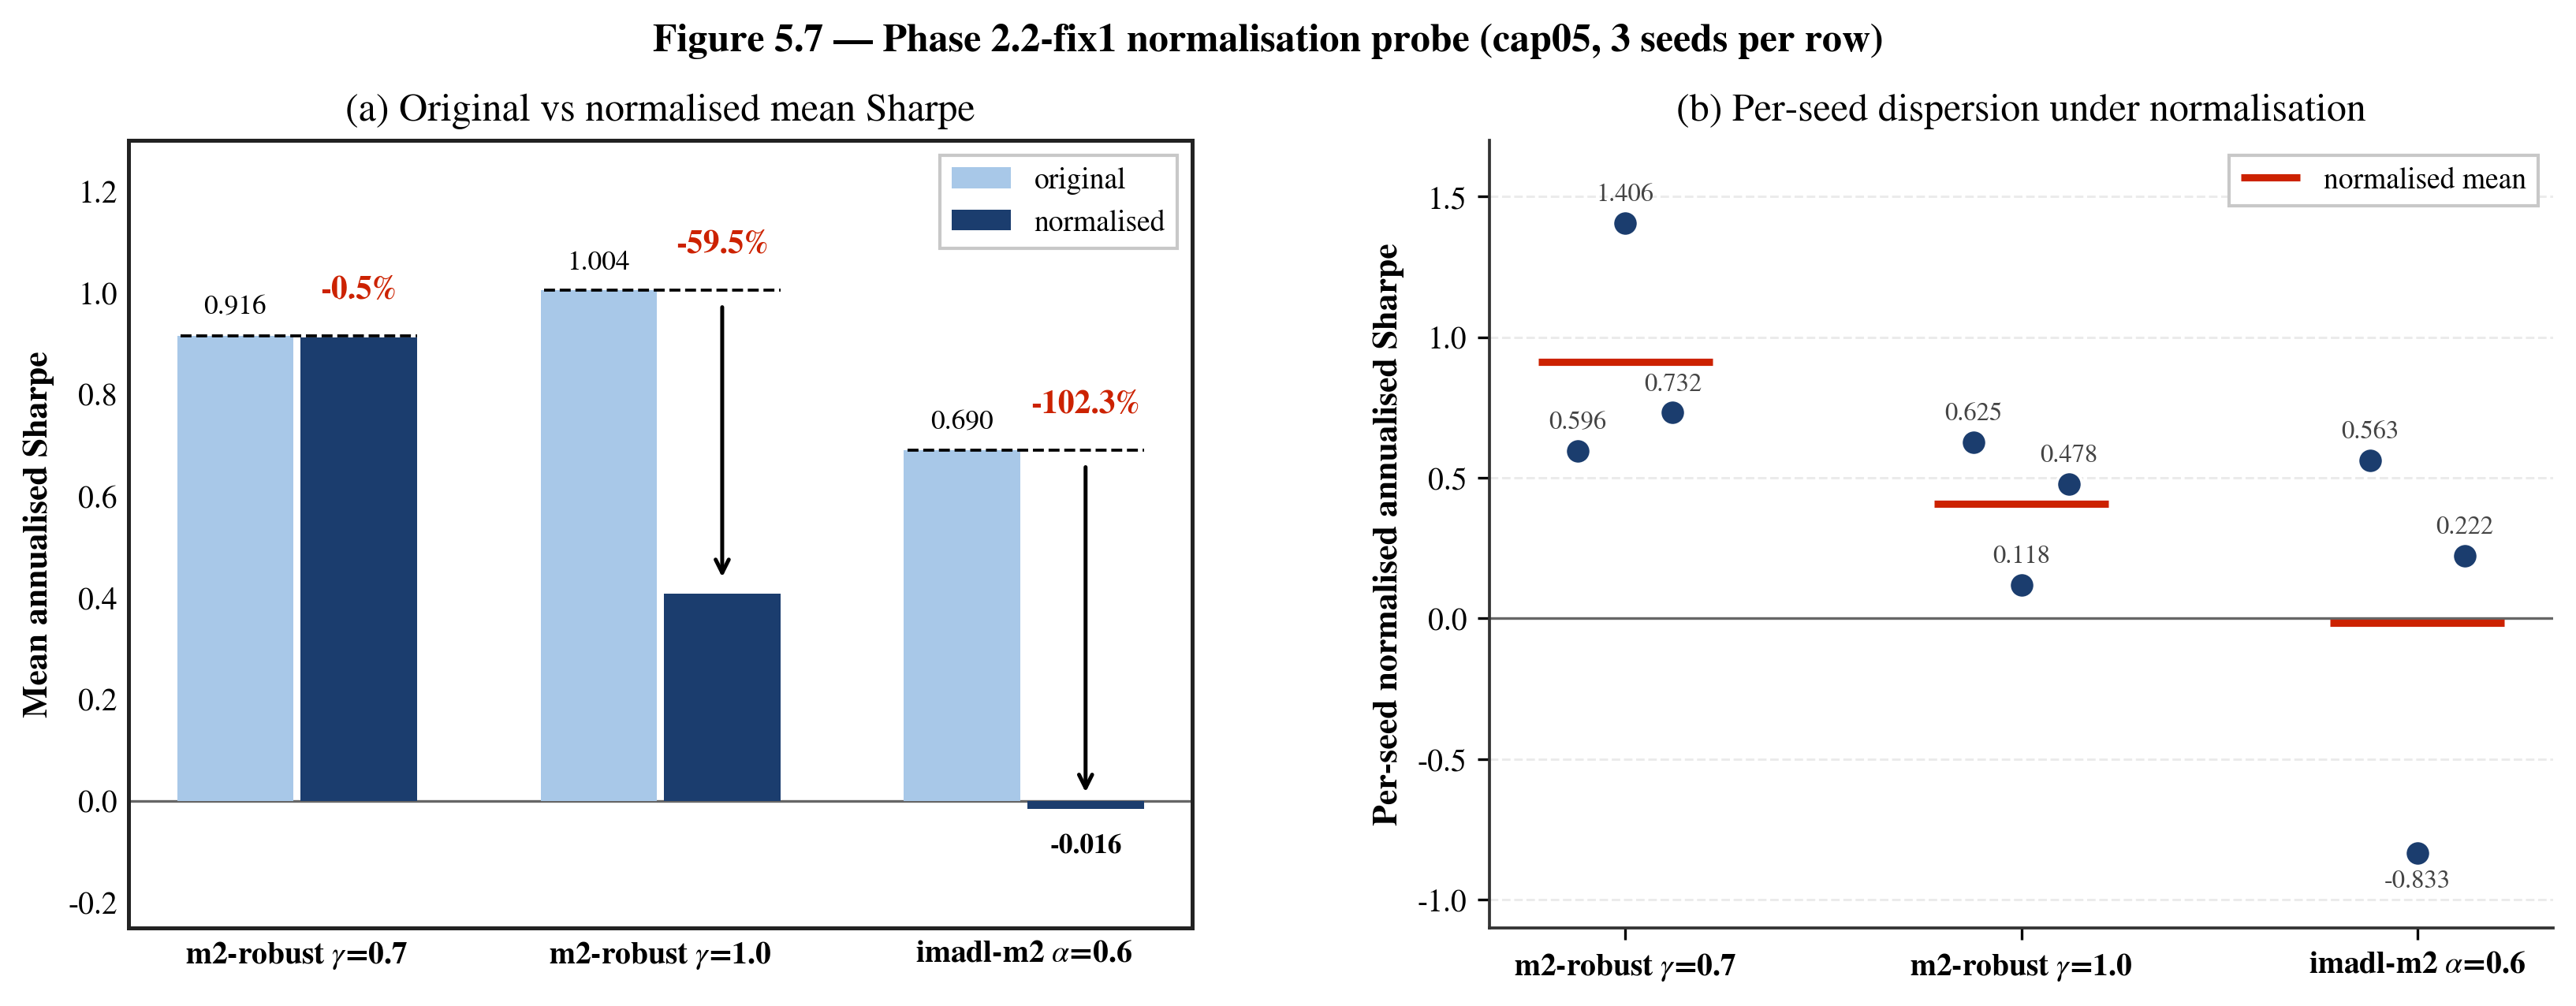
\includegraphics[width=0.9\textwidth]{figures/fig5_7_normalisation_probe.png}
\caption[Loss-component normalisation probe]{Loss-component normalisation probe. Left: grouped bar showing the original vs normalised mean annualised Sharpe for the three strongest candidates (\texttt{m2\_robust\_gamma07}, \texttt{m2\_robust\_gamma10}, \texttt{imadl\_m2\_alpha06}), 3 seeds per row. Right: per-seed normalised Sharpes (dots) and their mean (short horizontal bar) for each candidate. Evaluation window \texttt{1995-01..1996-12}, \texttt{cap05}. Scale ratios are diagnostics-estimated (per-component logger not yet implemented).}
\label{fig:normalisation-probe}
\end{figure}

Three points follow. First, normalisation is not a universal fix. Only \texttt{gamma07} is approximately stable under normalisation (mean Sharpe moves from $0.9156$ to $0.9112$, a change smaller than the per-seed dispersion in either configuration). Both \texttt{gamma10} and \texttt{alpha06} degrade materially -- by roughly a factor of two for \texttt{gamma10} and to near zero for \texttt{alpha06}. Normalisation therefore does not correct scale imbalance in a uniform way.

Second, the fact that \texttt{gamma07} is approximately stable under the diagnostic normalisation probe while \texttt{gamma10} and \texttt{alpha06} are not suggests that the observed \texttt{gamma07} Sharpe is not an artefact of the specific relative scale of the two loss components. Its signal is consistent across the original and diagnostic-normalised settings. By contrast, \texttt{gamma10}'s apparent edge in mean Sharpe without normalisation is sensitive to scale and should be treated as a contingent result.

Third, the probe itself has a known limitation: the scale ratios are estimated from logged diagnostics rather than measured directly through a per-component logger. The probe is therefore consistent with -- but not dispositive of -- a design claim that \texttt{gamma07} is approximately scale-stable. Chapter~6 flags this as a priority for future work.

In summary, component normalisation is informative but is not recommended as a blanket fix across the hybrid-multiplicative family. \texttt{gamma07} does not require it; \texttt{gamma10} and \texttt{alpha06} are damaged by it in the current evidence.

\section{Claim-boundary diagnostics}

\label{sec:claim-boundary-diagnostics}

Diagnostic passes confirm that cross-phase comparisons (e.g., stacking Phase~2 tables against Phase~3 tables) involve small but systematic runner and formula differences that are not attributable to a single factor. These differences do not invalidate controlled comparisons within a single phase, but they prevent claims of the form ``Phase~3 improves Phase~2 by $X$ Sharpe points.''

Two claim boundaries follow. First, \textbf{intra-phase comparison is strong}: within each table the loss function is the only varying factor. Second, \textbf{inter-phase comparison is moderate to weak}: cross-phase comparisons differ in seed set, parameterisation, and implementation details (see \S3.8). They are reasonable as design motivation but should not be quoted as direct-improvement claims. The closest supportable cross-phase statement is descriptive: the $\gamma$ family, once evaluated under multi-seed conditions, produces a mean Sharpe that exceeds the best Phase~2 seed-42 variant, but the two rows differ in more than one experimental factor.

\section{Headline findings and recommendations}

\label{sec:headline-findings}

Figure~\ref{fig:cumulative-return-paths} shows the cumulative long-short return paths that underlie the summary statistics in \S5.2--\S5.5. The left panel places the Phase~1 baselines in time: MSE and IMADL produce negative or flat paths throughout the 24-month window, while the hybrid variants (M1, A3) accumulate positive returns steadily. The right panel shows the Phase~2 gamma robustness picture: \texttt{gamma07} (red) produces the most consistent upward path across all three seeds, with a narrow seed envelope; \texttt{gamma10} (orange) reaches a higher peak in its best seed but shows wider dispersion; \texttt{gamma03} collapses early and never recovers.

\begin{figure}[H]
\centering

\includegraphics[width=0.9\textwidth]{figures/fig5_8_cumulative_return_paths.png}
\caption[Cumulative long-short return paths]{Cumulative long-short return paths. Left: Phase~1 baseline losses at seed 42; solid lines for hybrid variants, dashed for pure directional losses. Right: Phase~2 M2-robust $\gamma$ sweep; thick line is the mean across 3 seeds and shaded band is the min--max seed envelope. Train \texttt{1990-01..1994-12}, test \texttt{1995-01..1996-12}, \texttt{cap05}.}
\label{fig:cumulative-return-paths}
\end{figure}

The final loss recommendation rests on \S5.4--\S5.6, which together constitute the only multi-seed robustness evidence reported in this chapter. The recommendation has three tiers:

\textbf{Primary: \texttt{m2\_robust\_gamma07}.} Mean Sharpe $0.9156$, coefficient of variation $0.1808$, mean cumulative return $+27.99\%$ over 24 months, evaluated across three seeds on the \texttt{cap05} portfolio. Approximately stable under the diagnostic normalisation probe (normalised mean Sharpe $0.9112$). No seed in the run produces a negative Sharpe. This is the best-supported single choice for a loss function in the design space studied in this report.

\textbf{High-return alternative: \texttt{m2\_robust\_gamma10}.} Mean Sharpe $1.0043$ is the highest in the integrated sweep, but its coefficient of variation $0.5613$ is three times that of \texttt{gamma07}, its per-seed Sharpe range is wide ($0.4587$ to $1.5847$), and normalisation reduces its mean Sharpe to $0.4072$. It is appropriate only where the reader knowingly accepts high seed-sensitivity in exchange for a higher best-case Sharpe.

\textbf{Stable fallback: \texttt{imadl\_m2\_alpha06}.} Mean Sharpe $0.6895$, CV $0.2443$, mean cumulative return $+30.42\%$. This is the peak of the IMADL-m2 $\alpha$ sweep and its cumulative return is actually the largest of the three tiered candidates, though its Sharpe is lower than \texttt{gamma07}. It is selected as the stable fallback by its favourable stability/return trade-off rather than by Sharpe dominance, and it provides the next-best independent corroboration that a hybrid-multiplicative design with a robust component is the productive region of the loss space.

In summary, the empirical answer to the research questions posed in Chapter~1 is: within the static 24-month protocol studied here, a hybrid-multiplicative loss with a tuned robust component ($\gamma = 0.07$) outperforms traditional regression losses and pure absolute-loss variants on seed-42 same-window Sharpe, and among the competitive Phase~2 multi-seed rows it achieves the best joint Sharpe-stability profile, with a stable fallback available through the IMADL-m2 $\alpha$ family at the same order of Sharpe. Scope limitations are discussed in Chapter~6.

\cleardoublepage

\chapter{Conclusion}

\label{ch:conclusion}

\section{Summary of findings}

\label{sec:summary-of-findings}

This report conducted a controlled, single-factor study of loss-function design for cross-sectional stock-return prediction with a multi-layer perceptron. Within each comparison table, data, features, architecture, training protocol, portfolio construction, and evaluation metrics were fixed; only the loss function was varied. Under this protocol, the empirical evidence in Chapter~5 supports the following direct answers to the three research questions posed in Chapter~1.

\textbf{RQ1: How do prediction-level and portfolio-level metrics change when only the loss function is altered?} At the single-seed baseline (Chapter~5 \S5.2), prediction-level and portfolio-level metrics decouple substantially. Losses that produce extremely negative R² (the absolute-loss family) can still yield competitive portfolio Sharpes, because the portfolio depends on cross-sectional ranks rather than calibrated magnitudes. R² is therefore a scale diagnostic rather than a primary performance metric in this setting. Among baseline losses, the hybrid multiplicative variant \texttt{hybrid\_mul\_m1} produces the best single-seed Sharpe, motivating the hybrid-loss design direction that Phase 2 and Phase 3 extend.

\textbf{RQ2: Within the hybrid-loss design space, which combination of directional and robust components performs best on the joint Sharpe-stability criterion?} The multi-seed evidence (Chapter~5 \S5.4 and \S5.5, three seeds per row) identifies the M2-robust $\gamma$ family as the productive region of the loss space. This family augments the base multiplicative hybrid (M2) with an explicit prediction-variance penalty: $L = L_{\mathrm{M2}} + \gamma \cdot \mathrm{Var}(\hat y)$. Within that family, \texttt{m2\_robust\_gamma07} ($\gamma = 0.7$) achieves mean Sharpe $0.9156$ with coefficient of variation $0.1808$ and mean cumulative return $+27.99\%$ over 24 months. \texttt{m2\_robust\_gamma10} has a higher mean Sharpe ($1.0043$) but three times the CV, and its per-seed Sharpe range is wide ($0.4587$ to $1.5847$). The integrated sweep shows that the IMADL-m2 $\alpha$ family peaks at $\alpha = 0.6$ (mean Sharpe $0.6895$, CV $0.2443$), that the IMADL-GMADL $\beta$ family does not produce robust positive Sharpes (CV values from 4.0 to 139.5), and that the adaptive-$\lambda$ family underperforms both on Sharpe and on stability. \texttt{m2\_robust\_gamma07} emerges as the single best candidate on the joint Sharpe-stability criterion; \texttt{imadl\_m2\_alpha06} corroborates the multiplicative-hybrid direction from an independent parameterisation.

\textbf{RQ3: Are the observed winners approximately stable under the diagnostic loss-component normalisation probe?} The normalisation probe (Chapter~5 \S5.6) applies component normalisation to the three strongest candidates. \texttt{m2\_robust\_gamma07} is approximately flat under normalisation (mean Sharpe $0.9156 \to 0.9112$, a change smaller than the per-seed dispersion). Both \texttt{m2\_robust\_gamma10} ($1.0043 \to 0.4072$) and \texttt{imadl\_m2\_alpha06} ($0.6895 \to -0.0161$) degrade materially. The operational conclusion is that component normalisation is \emph{not} a universal fix, and that \texttt{m2\_robust\_gamma07} is the only one of the three candidates whose signal is approximately stable in the diagnostic normalisation probe. The probe itself acknowledges that its scale ratios are diagnostics-estimated rather than measured by a fully instrumented per-component logger; that limitation is recorded as a future-work item.

\textbf{Final recommendation.} Combining the answers to RQ1--RQ3, the report's final loss recommendation has three tiers:

\begin{itemize}
 \item \textbf{Primary: \texttt{m2\_robust\_gamma07}.} Mean Sharpe $0.9156$, CV $0.1808$, mean cumulative return $+27.99\%$. Approximately stable under the diagnostic component-normalisation probe. No seed in the run produces a negative Sharpe. This is the best-supported single choice.
 \item \textbf{High-return alternative with explicit caveat: \texttt{m2\_robust\_gamma10}.} Mean Sharpe $1.0043$, CV $0.5613$. Appropriate only where the user knowingly accepts seed-sensitivity in exchange for best-case Sharpe.
 \item \textbf{Stable fallback: \texttt{imadl\_m2\_alpha06}.} Mean Sharpe $0.6895$, CV $0.2443$, mean cumulative return $+30.42\%$. Provides independent corroboration that the multiplicative-hybrid region is the productive one.
\end{itemize}

\section{Limitations and future work}

\label{sec:limitations}

The findings are scoped by several design choices: a single US equity monthly panel, a fixed 24-month evaluation window (no rolling retraining), three random seeds per multi-seed row, a single frozen architecture (MLP[64,32,16]), one feature set (X1, 15 columns), and a gross-of-cost portfolio with fixed bucket thresholds. These constraints ensure clean internal validity but limit external generalisation. The most impactful extensions would be (1)~a rolling-window evaluation across market regimes, (2)~a larger seed depth ($\geq$10) for tighter confidence intervals, (3)~a per-component loss logger to replace the diagnostics-estimated scale ratios in the normalisation probe, and (4)~feature-set and asset-class sensitivity tests.

\section{Concluding remarks}

\label{sec:concluding-remarks}

Under the static 24-month protocol studied here, \texttt{m2\_robust\_gamma07} is the best-supported loss recommendation --- scoped to US equity monthly data, a single evaluation window, and three-seed evidence. The broader contribution is methodological: a controlled evidence protocol that isolates the loss function as a design variable and measures multi-seed stability alongside mean performance, providing a reusable template for future loss-design research.

\cleardoublepage

% === Appendices ===
\appendix
\chapter{Loss Function Definitions and Gradients}

\label{chap:loss-definitions}

This appendix expands the loss-family definitions from Chapter~3 \S3.3 with explicit closed-form expressions and derivatives with respect to the prediction $\hat y$. Every formula in Sections A.1--A.3.2 matches the implementation in \texttt{Model\_Train/losses.py} on the current \texttt{main} branch. Section~A.3.3 records the conceptual form used to interpret Phase~2 branch outputs; its exact closed form lives on the \texttt{phase2.2-fix} branch. Gradients are stated pointwise; the effective training gradient at each optimiser step is the batch average (or median for \texttt{MedSE}) of the pointwise gradient.

Throughout this appendix, $y$ is the scalar realised return, $\hat y$ is the scalar prediction, and $e = y - \hat y$ is the residual. Where a batch-normalisation factor appears, the batch-level mean is written $\mathbb{E}_{\mathcal{B}}[\cdot]$ and the small regulariser $\epsilon = 10^{-8}$ is included to avoid division by zero.

% ============================================================
\section{Regression Losses}

\label{sec:regression-losses}

\subsection{MSE}

\label{subsec:mse}

\begin{equation}
L_{\mathrm{MSE}}(y, \hat y) = (y - \hat y)^2,
\qquad
\frac{\partial L_{\mathrm{MSE}}}{\partial \hat y} = -2\,(y - \hat y).
\end{equation}

Batch reduction: arithmetic mean.

\subsection{MedSE}

\label{subsec:medse}

\begin{equation}
L_{\mathrm{MedSE}}(y, \hat y) = (y - \hat y)^2,
\qquad
\text{batch reduction} = \mathrm{median}.
\end{equation}

Because the median is non-decomposable, the gradient at each observation is zero at every observation \emph{except} those that determine the batch median. In PyTorch the autograd routes gradient only through the median-ranked observation; this is why MedSE training is inherently noisier and why \texttt{reduction="median"} is declared explicitly in \texttt{medse\_loss}.

\subsection{Huber (as magnitude backbone)}

\label{subsec:huber}

Used inside every hybrid loss, with $\delta = 0.01$ hard-coded in \texttt{\_huber\_term}:

\begin{equation}
H_\delta(e) =
\begin{cases}
\tfrac12 e^2 & |e| \le \delta, \\
\delta\, (|e| - \tfrac12 \delta) & |e| > \delta,
\end{cases}
\qquad
\frac{\partial H_\delta}{\partial \hat y}
=
\begin{cases}
-e & |e| \le \delta, \\
-\delta \cdot \operatorname{sgn}(e) & |e| > \delta.
\end{cases}
\end{equation}

The gradient is continuous in $e$ (the one-sided derivatives agree at both boundaries $|e| = \delta$) and bounded by $\delta$ in absolute value.

% ============================================================
\section{Directional Losses}

\label{sec:directional-losses}

\subsection{MADL (differentiable)}

\label{subsec:madl}

With $a = 25$ fixed:

\begin{equation}
L_{\mathrm{MADL}}(y, \hat y) = -\tanh(a \cdot y \cdot \hat y) \cdot |y|,
\end{equation}
\begin{equation}
\frac{\partial L_{\mathrm{MADL}}}{\partial \hat y} = -a \cdot y \cdot |y| \cdot \operatorname{sech}^2(a \cdot y \cdot \hat y).
\end{equation}

The gradient peaks near $a \cdot y \cdot \hat y = 0$ and decays exponentially as $|a \cdot y \cdot \hat y|$ grows. For realistically small $|y|$ (monthly returns typically a few per cent), the factor $y \cdot |y| = y^2 \cdot \operatorname{sgn}(y)$ is of order $10^{-4}$, which is the ``weak-gradient-near-zero'' behaviour described in Chapter~2 \S2.4.

\subsection{GMADL}

\label{subsec:gmadl}

With $a = 100$ and $b = 2$ fixed:

\begin{equation}
L_{\mathrm{GMADL}}(y, \hat y) = -\big[\sigma(a \cdot y \cdot \hat y) - \tfrac12\big] \cdot |y|^b,
\end{equation}
\begin{equation}
\frac{\partial L_{\mathrm{GMADL}}}{\partial \hat y}
= -a \cdot y \cdot |y|^b \cdot \sigma(a \cdot y \cdot \hat y) \cdot \big[1 - \sigma(a \cdot y \cdot \hat y)\big].
\end{equation}

The $|y|^b = y^2$ factor provides stronger magnitude weighting than MADL, but the sigmoid derivative $\sigma(1-\sigma)$ saturates at $|a y \hat y| \gg 1$. Together these explain why GMADL produces larger absolute prediction values (to push $|a y \hat y|$ into the saturation region) while preserving directional ranking --- and why average R\textsuperscript{2} values diverge under this loss (Chapter~5 \S5.2).

\subsection{IMADL (rebalanced)}

\label{subsec:imadl}

With $a = 100$, $b = 2$, $\lambda_{\mathrm{dir}} = \lambda_{\mathrm{mag}} = 1$ fixed:

\begin{equation}
D(y, \hat y) = \big[1 - \sigma(a\, y\, \hat y)\big] \cdot \frac{|y|^b}{\mathbb{E}_{\mathcal{B}}[|y|^b] + \epsilon},
\end{equation}
\begin{equation}
L_{\mathrm{IMADL}}(y, \hat y) = \lambda_{\mathrm{dir}} \cdot D(y, \hat y) + \lambda_{\mathrm{mag}} \cdot (y - \hat y)^2,
\end{equation}
\begin{multline}
\frac{\partial L_{\mathrm{IMADL}}}{\partial \hat y}
= -\lambda_{\mathrm{dir}} \cdot a\, y \cdot \sigma(a\, y\, \hat y) \cdot \big[1 - \sigma(a\, y\, \hat y)\big] \cdot \frac{|y|^b}{\mathbb{E}_{\mathcal{B}}[|y|^b] + \epsilon} \\
- 2\,\lambda_{\mathrm{mag}}\,(y - \hat y).
\end{multline}

The batch-normalisation factor $\mathbb{E}_{\mathcal{B}}[|y|^b]$ decouples the scale of the directional gradient from the particular batch composition; it is treated as a constant during the backward pass through that observation (for gradients with respect to $\hat y$, the normalisation denominator is constant, matching the design intent).

% ============================================================
\section{Hybrid Losses}

\label{sec:hybrid-losses}

\subsection{Additive (A-series)}

\label{subsec:additive}

With Huber $\delta = 0.01$ fixed and $(\lambda_{\mathrm{dir}}, \lambda_{\mathrm{hub}})$ varied per variant (see Chapter~3 \S3.3.3):

\begin{equation}
L_{\mathrm{add}}(y, \hat y) = \lambda_{\mathrm{dir}} \cdot D(y, \hat y) + \lambda_{\mathrm{hub}} \cdot H_\delta(y - \hat y),
\end{equation}
\begin{equation}
\frac{\partial L_{\mathrm{add}}}{\partial \hat y}
= \lambda_{\mathrm{dir}} \cdot \frac{\partial D}{\partial \hat y}
+ \lambda_{\mathrm{hub}} \cdot \frac{\partial H_\delta}{\partial \hat y}.
\end{equation}

Both components contribute additively to the gradient; the relative weighting is $(\lambda_{\mathrm{dir}}, \lambda_{\mathrm{hub}})$. The A-variants scan this 2-dimensional hyperparameter.

\subsection{Multiplicative (M-series)}

\label{subsec:multiplicative}

\begin{equation}
L_{\mathrm{mul}}(y, \hat y) = \big(1 + \lambda_{\mathrm{dir}} \cdot D(y, \hat y)\big) \cdot H_\delta(y - \hat y),
\end{equation}
\begin{equation}
\frac{\partial L_{\mathrm{mul}}}{\partial \hat y}
= \lambda_{\mathrm{dir}} \cdot \frac{\partial D}{\partial \hat y} \cdot H_\delta(y - \hat y)
+ \big(1 + \lambda_{\mathrm{dir}} \cdot D(y, \hat y)\big) \cdot \frac{\partial H_\delta}{\partial \hat y}.
\end{equation}

The multiplicative form couples the two components: the Huber gradient is \emph{gated} by the directional factor $1 + \lambda_{\mathrm{dir}} D$. When the direction is predicted correctly, $D \to 0$ and the gradient reduces to $\partial H_\delta / \partial \hat y$. When the direction is predicted wrongly, the sigmoid penalty $\sigma(ay\hat y)$ approaches 0 so $[1-\sigma(\cdot)]$ approaches 1, and the Huber gradient is amplified by a factor of $1 + \lambda_{\mathrm{dir}} \cdot D$, where $D$ is proportional to the batch-normalised magnitude weight $|y|^b / (\mathbb{E}_{\mathcal{B}}[|y|^b]+\epsilon)$.

\subsection{M2-robust \texorpdfstring{$\gamma$}{gamma} family}

\label{subsec:m2-robust}

Conceptually, the M2-robust loss replaces the fixed-threshold Huber backbone with a $\gamma$-controlled saturating magnitude term $H^{\gamma}(e)$ and combines it with the same directional-gating structure:

\begin{equation}
L_{\mathrm{M2\text{-}robust},\gamma}(y, \hat y) = \big(1 + \lambda_{\mathrm{dir}} \cdot D(y, \hat y)\big) \cdot H^{\gamma}(y - \hat y).
\end{equation}

The robustness schedule $H^{\gamma}(e)$ is a smooth monotone function that approaches $\tfrac12 e^2$ for small $|e|$ and saturates above a threshold controlled by $\gamma$. Small $\gamma$ flattens the loss surface and prioritises the directional component; large $\gamma$ recovers a nearly unbounded quadratic behaviour. The $\gamma$ refinement of Chapter~5 \S5.4 scans $\gamma \in \{0.03, 0.05, 0.07, 0.10, 0.15\}$. The exact closed form used in the Phase~2.2 runner lives on the \texttt{phase2.2-fix} branch together with the runner scripts; the empirically selected setting within the reported 24-month, 3-seed protocol is $\gamma = 0.07$ (see Chapter~5 \S5.4 and Table~5.3).

% ============================================================
\section{Notes on Practical Implementation}

\label{sec:practical-notes}

Two implementation points are worth repeating for completeness, both documented in \texttt{Model\_Train/losses.py}:

\begin{enumerate}
    \item \textbf{Reduction.} Every loss function uses \texttt{reduction="mean"} by default, except MedSE which uses \texttt{reduction="median"}. Passing \texttt{reduction="none"} returns the pointwise loss vector, which the tests in \texttt{tests/} consume.
    \item \textbf{Numerical guards.} IMADL and the hybrid variants use the batch-mean normalisation $\mathbb{E}_{\mathcal{B}}[|y|^b] + \epsilon$ with $\epsilon = 10^{-8}$; the Huber term has no special numerical guard because it is smooth and bounded.
\end{enumerate}

\cleardoublepage

\chapter{Per-Seed Raw Results and Reproducibility}

\label{ch:per-seed-raw-results}

This appendix tabulates the per-seed raw Sharpes that the multi-seed grouped summaries in Chapter~5 aggregate, so that the reader can verify the mean, standard deviation, and coefficient of variation directly. It also lists the exact reproduction commands for every table in Chapter~5.

\section{Phase 2.2 $\gamma$ refinement --- per-seed annualised Sharpe}

\label{sec:phase22-gamma-refinement-per-seed}

Source: \texttt{doc/phase2-fix/phase2\_2/gamma\_refinement/reports/phase2\_raw\_runs.csv}. Static train \texttt{1990-01..1994-12}, test \texttt{1995-01..1996-12}, \texttt{cap05} portfolio cap. Three seeds per $\gamma$; seeds are \texttt{\{42, 52, 62\}}.

\textbf{Table B.1 --- Phase 2.2 $\gamma$ refinement per-seed annualised Sharpe.}

\begin{table}[H]\centering
\caption{Phase 2.2 $\gamma$ refinement per-seed annualised Sharpe}\label{tab:b1-gamma-per-seed}
\begin{tabular}{ccccccc}\toprule
Loss & seed 42 & seed 52 & seed 62 & mean & std & CV \\\midrule
\texttt{m2\_robust\_gamma03} & $-0.01987$ & $0.32631$ & $0.66380$ & $0.32341$ & $0.34184$ & $1.05698$ \\
\texttt{m2\_robust\_gamma05} & $0.86960$ & $0.66697$ & $0.57964$ & $0.70540$ & $0.14875$ & $0.21087$ \\
\texttt{m2\_robust\_gamma07} & $0.90972$ & $1.08404$ & $0.75316$ & $0.91564$ & $0.16552$ & $0.18077$ \\
\texttt{m2\_robust\_gamma10} & $0.45873$ & $1.58465$ & $0.96958$ & $1.00432$ & $0.56376$ & $0.56134$ \\
\texttt{m2\_robust\_gamma15} & $0.90214$ & $0.40845$ & $1.13823$ & $0.81627$ & $0.37239$ & $0.45621$ \\
\bottomrule\end{tabular}
\end{table}

(The seed-42 \texttt{m2\_robust\_gamma07} row here, Sharpe $0.90972$, differs from the rounded $0.9156$ grouped-summary mean because the grouped row averages the three per-seed values. Both numbers trace to the raw CSV.)

\section{Phase 2.2-fix1 normalisation probe --- per-seed annualised Sharpe}

\label{sec:phase22-fix1-normalisation-per-seed}

Source: \texttt{doc/phase2-fix/phase2.2-fix1/phase2\_summary.json}.

\textbf{Table B.2 --- Phase 2.2-fix1 normalisation probe per-seed Sharpe.}

\begin{table}[H]\centering
\caption{Phase 2.2-fix1 normalisation probe per-seed Sharpe}\label{tab:b2-norm-probe-per-seed}
\begin{tabular}{cccccc}\toprule
Loss & Normalised seed 1 & Normalised seed 2 & Normalised seed 3 & Normalised mean & Original mean \\\midrule
\texttt{m2\_robust\_gamma07} & $0.5956$ & $1.4064$ & $0.7317$ & $0.9112$ & $0.9156$ \\
\texttt{m2\_robust\_gamma10} & $0.6254$ & $0.1181$ & $0.4780$ & $0.4072$ & $1.0043$ \\
\texttt{imadl\_m2\_alpha06} & $0.5628$ & $-0.8335$ & $0.2224$ & $-0.0161$ & $0.6895$ \\
\bottomrule\end{tabular}
\end{table}

(The per-seed IDs are anonymised in the summary JSON. The project notes record that the normalisation probe re-uses the same three seeds as the $\gamma$ refinement, but the mapping between the numeric position and \texttt{\{42, 52, 62\}} is not preserved in the summary file; the mean and per-seed spread remain the relevant quantities.)

\section{Phase 2 integrated summary --- grouped row summary (reproduction)}

\label{sec:phase2-integrated-summary}

Source (read without switching branches): \texttt{git show phase2.2-fix:doc/phase2-fix/reports/phase2\_grouped\_summary.csv}.

Grouped rows quoted in Chapter~5 Table~5.4 are read directly from this CSV (column-by-column, no averaging or post-processing). Per-seed raw rows for the same variants are available in the sibling \texttt{phase2\_raw\_runs.csv} on the same branch. Per-seed detail is elided from the main text for readability, but every seed is recoverable via:

\begin{lstlisting}[language=bash]
git show phase2.2-fix:doc/phase2-fix/reports/phase2_raw_runs.csv
\end{lstlisting}

\section{Reproduction commands per Chapter~5 table}

\label{sec:reproduction-commands}

Tables 5.1--5.2 reproduce on \texttt{main} at commit \texttt{6c0fbde} with the repository-root data CSVs (\texttt{*.csv} matching the \texttt{-{}-pattern}) and the shared \texttt{best\_hyperparameters.txt}. Tables 5.3--5.5 are read or reproduced from the \texttt{phase2.2-fix} branch and \texttt{doc/phase2-fix/phase2.2-fix1/} artifacts as listed below.

\subsection{Table 5.1 --- Baseline losses (seed 42, 24 months)}

\label{ssec:table51-baseline-losses}

For each \texttt{\{loss\} in \{mse, medse, madl, gmadl, imadl, hybrid\_mul\_m1, hybrid\_mul\_m2\}}:

\begin{lstlisting}[language=bash]
python run_sanity_check_{loss}.py \
  --data-dir . \
  --pattern '*.csv' \
  --train-start 1990-01 \
  --train-end 1994-12 \
  --test-start 1995-01 \
  --test-months 24 \
  --max-epochs 20 \
  --batch-size 1024 \
  --best-config-path best_hyperparameters.txt \
  --output-dir <output-root>/results/baseline/{loss} \
  --seed 42
\end{lstlisting}

The output CSV at \texttt{<output-root>/results/baseline/\{loss\}/sanity\_metrics\_\{loss\}.csv} must have \texttt{row\_count = 24}, \texttt{first\_month = 1995-01}, \texttt{last\_month = 1996-12}. The paired summary JSON is at \texttt{sanity\_summary\_\{loss\}.json}.

\subsection{Table 5.2 --- Phase 1.5 A/M variants (seed 42, 24 months)}

\label{ssec:table52-phase15-variants}

For each variant (\texttt{A1..A5}, \texttt{M1..M4}) use the corresponding runner, e.g., for \texttt{M2}:

\begin{lstlisting}[language=bash]
python run_sanity_check_hybrid_mul_m2.py \
  --data-dir . --pattern '*.csv' \
  --train-start 1990-01 --train-end 1994-12 \
  --test-start 1995-01 --test-months 24 \
  --max-epochs 20 --batch-size 1024 \
  --best-config-path best_hyperparameters.txt \
  --output-dir <output-root>/results/phase15/M2 \
  --seed 42
\end{lstlisting}

The runner-to-variant mapping is listed in \texttt{doc/final\_report\_all\_24m\_evidence/manifests/run\_manifest.json}.

\subsection{Table 5.3 --- Phase 2.2 $\gamma$ refinement (multi-seed)}

\label{ssec:table53-gamma-refinement-multiseed}

The $\gamma$ refinement was run from the \texttt{phase2.2-fix} branch with three seeds and the five $\gamma$ values listed in \S\ref{sec:phase22-gamma-refinement-per-seed}. The grouped summary is reproduced locally at:

\begin{lstlisting}[language=bash]
doc/phase2-fix/phase2_2/gamma_refinement/reports/phase2_grouped_summary.csv
doc/phase2-fix/phase2_2/gamma_refinement/reports/phase2_raw_runs.csv
\end{lstlisting}

The per-seed raw CSV can be aggregated into the grouped summary by:

\begin{lstlisting}[language=Python]
import pandas as pd
raw = pd.read_csv("doc/phase2-fix/phase2_2/gamma_refinement/reports/phase2_raw_runs.csv")
grouped = (
    raw[raw["cap_tag"] == "cap05"]
    .groupby("loss")["long_short_sharpe"]
    .agg(["mean", "std", "min", "max", "count"])
)
grouped["cv"] = grouped["std"] / grouped["mean"].abs()
\end{lstlisting}

\subsection{Tables 5.4 and 5.5 --- Phase 2 integrated and normalisation}

\label{ssec:table54-55-phase2-integrated}

The integrated grouped summary is on branch \texttt{phase2.2-fix}:

\begin{lstlisting}[language=bash]
git show phase2.2-fix:doc/phase2-fix/reports/phase2_grouped_summary.csv
\end{lstlisting}

The normalisation probe summaries are on \texttt{main} at:

\begin{lstlisting}
doc/phase2-fix/phase2.2-fix1/phase1_summary.json
doc/phase2-fix/phase2.2-fix1/phase2_summary.json
\end{lstlisting}

\section{Reproducibility checklist}

\label{sec:reproducibility-checklist}

Before re-running any table for publication, verify:

\begin{enumerate}
\item Working directory is the repository root; \texttt{*.csv} data files are present.
\item \texttt{best\_hyperparameters.txt} is unchanged from commit \texttt{6c0fbde} (MLP[64, 32, 16], ReLU, dropout 0.2, input\_dim 15).
\item Python version $\geq$ 3.10; PyTorch installed; NumPy/pandas/matplotlib available for figure scripts.
\item CUDA or MPS accelerator is available if matching Phase 2 run behaviour (device auto-detection in \texttt{sanity\_check\_signal\_tilted.detect\_device}). CPU-only runs are numerically close but not bit-identical.
\item The runner CLI arguments match exactly (\texttt{-{}-test-months 24}, \texttt{-{}-train-start 1990-01}, \texttt{-{}-train-end 1994-12}, \texttt{-{}-test-start 1995-01}, \texttt{-{}-seed 42} for single-seed tables).
\item After each run, verify the output CSV has 24 rows with first month \texttt{1995-01} and last month \texttt{1996-12}; this is automated by the \texttt{*\_verification.json} writer in the evidence scripts.
\end{enumerate}

\section{Known numerical caveats}

\label{sec:known-numerical-caveats}

\begin{itemize}
\item CUDA non-determinism. \texttt{torch.backends.cudnn.deterministic} is not forced; bit-level reproduction across hardware is not guaranteed. Grouped-summary values in Chapter~5 are reported to be stable across re-runs within the same environment, but no formal rerun artifact has been preserved.
\item Floating-point noise in \texttt{compute\_portfolio\_returns}. The capped-simplex projection iterates up to 10 times; edge cases (multiple weights hitting the cap simultaneously) can produce microscopic differences across runs.
\item \texttt{git show phase2.2-fix:...} depends on the \texttt{phase2.2-fix} branch being present in the local clone. \texttt{git fetch} if needed.
\item The 6-month legacy window \texttt{1995-01..1995-06} in \texttt{sanity\_outputs/} is not part of this appendix's reproduction and should not be used for any final-report table.
\end{itemize}

\section{Complete model input columns}

\label{sec:complete-model-input-columns}

\textbf{Table B.3 --- Complete 15-column model input for X1.}

\begin{table}[H]\centering
\caption{Complete 15-column model input for X1}\label{tab:b3-model-input-columns}
\begin{tabular}{ccc}\toprule
\# & Column & Description \\\midrule
1 & RET & raw monthly total return for month $t$ \\
2 & VOL & monthly trading volume (shares) for month $t$ \\
3 & SHROUT & shares outstanding (thousands) for month $t$ \\
4 & r & numeric copy of RET \\
5 & to & monthly turnover = VOL/(SHROUT$\times$1000) \\
6 & cr\_1m & 1-month cumulative lagged return \\
7 & co\_1m & 1-month cumulative lagged turnover \\
8 & cr\_3m & 3-month cumulative lagged return \\
9 & co\_3m & 3-month cumulative lagged turnover \\
10 & cr\_6m & 6-month cumulative lagged return \\
11 & co\_6m & 6-month cumulative lagged turnover \\
12 & cr\_9m & 9-month cumulative lagged return \\
13 & co\_9m & 9-month cumulative lagged turnover \\
14 & cr\_12m & 12-month cumulative lagged return \\
15 & co\_12m & 12-month cumulative lagged turnover \\
\bottomrule\end{tabular}
\end{table}

\cleardoublepage

% === Bibliography ===
\bibliographystyle{plainnat}
\bibliography{references}
\cleardoublepage

\end{document}
